\documentclass[11pt,a4paper,oneside]{report}

\usepackage[margin=2.5cm]{geometry}
\usepackage{amsmath,amssymb,bm}
\usepackage[numbers,sort&compress]{natbib}
\usepackage{graphicx}
\usepackage{booktabs}
\usepackage{tabularx}
\usepackage{setspace}
\usepackage{microtype}
\usepackage{xcolor}
\usepackage{enumitem}
\usepackage[hidelinks]{hyperref}

\graphicspath{{figures/}}
\onehalfspacing
\setlength{\parskip}{0.32em}
\setlength{\parindent}{1.15em}
\setlist[itemize]{topsep=0.2em,itemsep=0.12em}
\setlist[enumerate]{topsep=0.2em,itemsep=0.12em}

\newcommand{\tagproposed}{\texttt{proposed}}
\newcommand{\tagsmoke}{\texttt{smoke-tested}}
\newcommand{\tagvalid}{\texttt{validated}}
\newcommand{\tagmatch}{\texttt{matched}}
\newcommand{\taginvalid}{\texttt{invalid}}
\newcommand{\stillreq}{\texttt{still required}}

\title{Staged predictive modelling of PEGDA\\
free-radical photopolymerization}
\author{Matthias Wessling\\[0.4em]
{\large Master's-thesis-style final report}\\[0.3em]
{\normalsize AVT.CVT --- Photopolymerization modelling campaign}\\[0.2em]
{\normalsize RWTH Aachen University}}
\date{13 September 2026}

\begin{document}
\maketitle

\begin{abstract}
\noindent
This report is a master's-thesis-style account of a staged campaign to predict acrylate conversion, operational gelation, and loop-aware hydrogel modulus for poly(ethylene glycol) diacrylate (PEGDA) photopolymerization without treating those quantities as a single dose number.
The locked scientific object is chain-growth free-radical polymerization driven by a prescribed irradiance history, later a digital micromirror surface field and Beer--Lambert attenuation, later plug flow, and finally a Macosko--Miller network post-processor with intramolecular loops.
Production Type~I kinetics follow Montgomery, Hamel, Skovran and Qi (\emph{Extreme Mechanics Letters}, 2022) for PEGDA~$250$ / Irgacure~819.
Projection uses their Gaussian pixel kernel as a fallback, not as a measured point-spread function.
Plug flow uses a \emph{separate} constitutive book taken from Slutzky, Stone and Nunes (\emph{Soft Matter}, 2019) for a PEGDA~$575$ jet.
Network mechanics follow Zhu, Yang, Genin, Lu, Xu and Lin (\emph{Journal of the Mechanics and Physics of Solids}, 2020), with eosin~Y bleaching ordinary differential equations switched off.
The high-fidelity species model of Dobson and Bowman (\emph{Advanced Functional Materials}, 2024) is a reference ontology, not the everyday right-hand side.

Seven stages (0--6) were implemented in a Python package under \texttt{src/photopolymerization/}, each with a frozen configuration, forward run, named validator, tests, overview figure, and journal tag.
As of 13~September~2026 all seven stages are internally \texttt{validated}.
None is \texttt{matched} to Fourier-transform infrared conversion, a camera kernel, an experimental critical speed, or rheology.
Dissolved oxygen in the Montgomery book remains \texttt{still required}.
Internal findings that survive those caveats include failed equal-dose reciprocity in the Montgomery closures, recovery of Slutzky's oxygen--monomer identity during induction, a grayscale interface width that is dominated by the optical kernel rather than Table~3 radical diffusion on an eight-second strip, numerical agreement of a Fig.~3-style jet with $M/M_0\simeq0.86$, and a loop-reduced elastically active fraction $\eta=0.378$ at full conversion for 20~vol\% PEGDA with Zhu's fitted loop parameter.

The report is not a printer manual and not a claim that in-house AVT resin equals any of the three literature formulations.
The recommended next scientific step is a Stage~1 FTIR overlay on a named recipe with a pre-declared error band.
\end{abstract}

\tableofcontents
\listoffigures
\listoftables

\chapter{Introduction}
\label{ch:intro}

\section{Motivation}

This report is a master's-thesis-style account of a staged modelling campaign for \emph{free-radical photopolymerization of poly(ethylene glycol) diacrylate} (PEGDA).
The engineering context is continuous-flow digital lithography of multi-porosity hydrogel patches, as envisaged in the DFG proposal \emph{Continuous-Flow Digital Lithography of Multi-Porosity Hydrogel Patches} (AVT.CVT, RWTH Aachen).
The scientific problem is older and more elementary than that device: given a known light history, and later a known flow, can one predict how many acrylate groups have reacted, whether a sample-spanning network exists, and how stiff the gel is---without treating those three questions as the same number?

A machine operator can print without answering them.
A working curve relating cure depth to the logarithm of dose \citep{Jacobs1992book} is a calibration for a given resin, lamp, and speed.
It is not a constitutive law.
Two parcels of resin can receive the same
\begin{equation}
  E = \int I(t)\,\mathrm{d}t
\end{equation}
and still differ in conversion $p$, gelation, and modulus, because bimolecular termination and oxygen inhibition make the outcome depend on the \emph{shape} of $I(t)$ \citep{Wydra2014,Lin2019,Dobson2024}.
A flowing jet continuously replenishes oxygenated liquid \citep{Slutzky2019}.
A DMD pixel is not a top-hat of light \citep{Montgomery2022,Meenakshisundaram2020}.
A dilute PEGDA solution may never gel even at full acrylate conversion, because too many additions close loops \citep{Zhu2020}.

The campaign therefore refuses a single mixed three-dimensional code on day one.
It implements seven stages (0--6), each with a frozen configuration, a forward run, named pass/fail gates, and one evidence tag (\texttt{proposed}, \texttt{smoke-tested}, \texttt{validated}, \texttt{matched}, or \texttt{invalid}).
As of 13 September 2026, Stages~0--6 are \tagvalid{} internally.
None is \tagmatch{} to FTIR, a camera point-spread function, an experimental critical speed, or rheology.

\section{Locked scientific object and non-goals}

\paragraph{Object.}
PEGDA \emph{chain-growth} free-radical photopolymerization: prescribed irradiance $I(t)$ maps to conversion $p$; later a DMD surface field and Beer--Lambert attenuation; later plug flow; then a loop-aware network post-processor $\eta(p,[\mathrm{PEGDA}]_0)$ and phantom modulus $G$.

\paragraph{Non-goals (parked).}
The full multi-species free-volume model of \citet{Dobson2024} as an everyday right-hand side; Navier--Stokes coupled to gelation; scattering optics; inverse DMD design; PNIPAM and thiol--ene closures; mixing eosin~Y Type~II bleaching ODEs into an Irgacure Type~I rate law; using a Jacobs working curve as the polymer state.

\paragraph{Two velocities.}
Pattern velocity $\mathbf{v}_{\mathrm{pattern}}$ (scan or mask) is independent of resin velocity $\mathbf{u}$.
A fluid element sees $\mathbf{v}_{\mathrm{pattern}}-\mathbf{u}$ \citep{Meenakshisundaram2020,Slutzky2019}.

\section{Intended reader}

The text is written for a starting graduate student who knows physical chemistry and transport but need not have worked on vat photopolymerization.
Jargon is defined once.
Evidence tags are used in the same sense throughout: engineering success (the solver finished) is not scientific validity.

\section{How this report is organised}

Chapter~\ref{ch:background} is the ontology: species, rates, light, oxygen, flow, and network, and the list of quantities that must not be identified.
Chapter~\ref{ch:literature} is a literature study of the five campaign papers and the supporting oxygen, reciprocity, and gelation literature, including the gap that the code was written to close.
Chapter~\ref{ch:methods} describes the Python package, the campaign quartet, numerical methods, and parameter books.
Chapter~\ref{ch:results} reports Stages~0--6 with gates, figures, and what each stage is \emph{not}.
Chapter~\ref{ch:matching} states what would be required to retag any stage \tagmatch.
Chapter~\ref{ch:conclusions} summarises findings, limitations, and parked work.

\section{Statement of originality and limitations}

No new laboratory experiment is reported.
The contribution is a citable modelling stack with separate chemistry keys, internal gates, and an explicit refusal to mix recipes.
Where a paper figure is reproduced only qualitatively (Montgomery Fig.~3-style Gaussians; Slutzky Figs.~2--3 illustrations), the tag remains \tagvalid, not \tagmatch.
Publisher PDFs in \texttt{Literature/} are local-only and are not redistributed.

% Auto-extracted from background_photopolymerization.tex (body only)
\chapter{Chemical and process background}
\label{ch:background}

This chapter is the chemistry and process ontology of the campaign.
It is written for a reader with undergraduate physical chemistry and transport who has not necessarily worked on stereolithography.
Quantitative claims about a specific PEGDA formulation remain \stillreq{} until they are taken from a named experiment or paper figure under the same recipe.
Figures in this chapter are teaching cartoons, not experimental measurements.

\section{What we are trying to predict}

A photopolymerizable liquid is a mixture that stays liquid in the dark and becomes a covalently connected solid (a gel or a densely crosslinked plastic) where and when it is illuminated, provided enough of the right chemical events occur.
The engineering goal is to \emph{place} that solid: in a vat printer, as a layer of a part; in a microfluidic channel, as a fiber or a patch; in a hydrogel, as a spatial map of stiffness.

A tempting one-number description is the \emph{dose}
\begin{equation}
  E = \int I(t)\,\mathrm{d}t,
  \label{eq:dose}
\end{equation}
where $I$ is the irradiance (energy, or moles of photons, arriving per area per time) at a point on the resin.
Stereolithography practice has long used a threshold form of this idea: a working curve relating cure depth to $\ln(E/E_c)$ \citep{Jacobs1992book}.
That description is useful as a machine calibration for a \emph{given} resin, optics, and speed.
It is not a material state.
Two parcels of resin can receive the same $E$ and still differ in how many acrylate groups have reacted, whether a sample-spanning network exists, and how stiff the gel is.
The rest of this note explains why, by naming the chemical inventory, the competing rates, the transport of light and oxygen, and the difference between chemical conversion and a mechanically active network.

\paragraph{PEGDA as the running example.}
Poly(ethylene glycol) diacrylate (PEGDA) is a short chain with an acrylate group at each end.
Each acrylate carries a carbon--carbon double bond that can add to a radical.
Because there are two such groups per molecule, chain growth can connect different PEGDA molecules into a branched, then crosslinked, network \citep{Zhu2020,Montgomery2022,Slutzky2019}.
PEGDA is \emph{not} one resin: molecular weight (for example $\approx 250$ versus $\approx 575\,\mathrm{g\,mol^{-1}}$), water content, photoinitiator, and atmosphere change both the kinetics and the gel point.
Numbers fitted to one formulation must not be treated as universal PEGDA constants.

\section{The chemical inventory}

Figure~\ref{fig:species} is a cartoon of the species that matter for a typical free-radical acrylate photopolymerization.
Light does not ``glue PEGDA together'' in one step.
Light is absorbed by a \emph{photoinitiator}.
The initiator produces \emph{radicals}.
Radicals add to acrylate double bonds (\emph{propagation}), which is the step that consumes monomer and builds polymer.
Radicals also destroy one another (\emph{termination}) and are scavenged by dissolved oxygen (\emph{inhibition}).
Only the competition among these processes decides how much conversion occurs for a given illumination.

\begin{figure}[htbp]
  \centering
  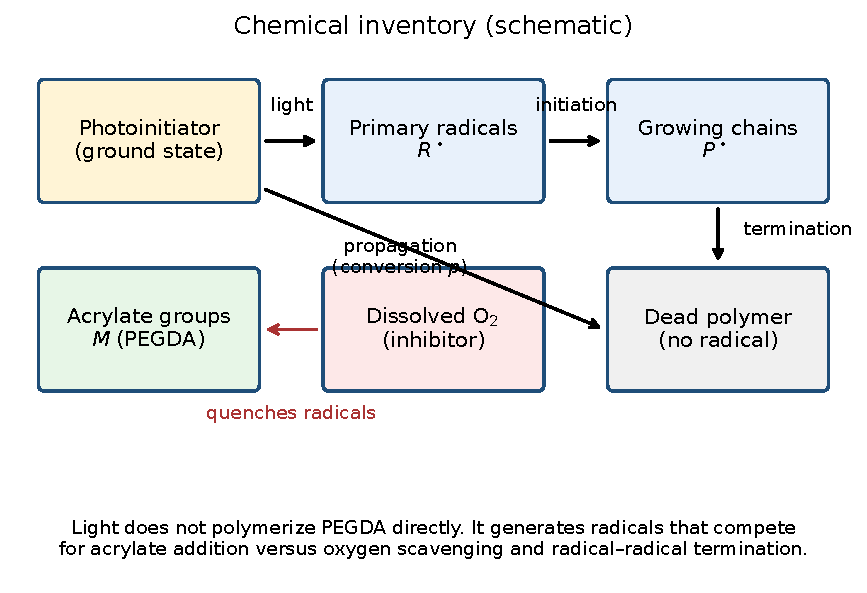
\includegraphics[width=0.98\textwidth]{fig_background_species.pdf}
  \caption{Schematic chemical inventory for a free-radical PEGDA photopolymerization.
  Boxes are species classes, not a complete kinetic scheme.
  Conversion $p$ counts reacted acrylate groups; it is not yet gelation or modulus.}
  \label{fig:species}
\end{figure}

\subsection{Photoinitiators: Type~I versus Type~II}

Photoinitiators are classified by how they generate the first radicals after absorbing a photon \citep{Dadashi2016,Zhu2020}.

\begin{description}
  \item[Type~I]
    A single molecule undergoes bond cleavage and yields (typically two) initiating radicals.
    Irgacure~819 (phenylbis(2,4,6-trimethylbenzoyl)phosphine oxide), used by \citet{Montgomery2022} and in the illustrations of \citet{Dobson2024}, is in this class.
    A compact description of photolysis is
    \begin{equation}
      \mathrm{PI} + n\,h\nu \;\longrightarrow\; 2\,R^\bullet,
      \label{eq:typeI}
    \end{equation}
    with a rate proportional to the local irradiance and to the remaining initiator concentration \citep{Montgomery2022}.
  \item[Type~II]
    The absorber is excited to a triplet and must react with a co-initiator (often an amine) to produce radicals.
    Eosin~Y with triethanolamine, the system of \citet{Zhu2020}, is Type~II.
    The excited dye can also return to the ground state or be irreversibly bleached to a leuco product.
    Bleaching therefore changes \emph{both} the initiation rate \emph{and} the optical absorption of the sample as curing proceeds.
\end{description}

These are different chemical objects.
A rate law written for Irgacure cleavage is not interchangeable with an eosin~Y bleaching cascade, even if both are used to cure PEGDA.

\subsection{Monomer, conversion, and what FTIR actually measures}

Let $[M]$ be the molar concentration of unreacted acrylate \emph{functional groups} (not necessarily the concentration of PEGDA molecules).
The degree of conversion is
\begin{equation}
  p(t) = 1 - \frac{[M](t)}{[M]_0}.
  \label{eq:conversion}
\end{equation}
In practice $p$ is often inferred from the decay of the infrared acrylate band relative to an internal carbonyl standard \citep{Montgomery2022}.
That measurement reports \emph{how many double bonds have disappeared}.
It does not, by itself, report whether those additions connected two different chains or closed a loop on the same chain, nor whether the sample has gelled.

\subsection{Radicals as a short-lived catalyst, not a stored dose}

The radical concentration $[R^\bullet]$ is typically orders of magnitude smaller than $[M]$ or $[\mathrm{O}_2]$.
Radicals are generated by initiation and lost by termination and inhibition.
If generation and loss nearly balance, one may write a quasi-steady estimate such as
\begin{equation}
  [R^\bullet] \approx \sqrt{\frac{R_i}{2k_t}}
  \label{eq:qss}
\end{equation}
in the oxygen-free, bimolecular-termination limit, with $R_i$ the initiation rate and $k_t$ the termination coefficient \citep{Zhu2020}.
Equation~\eqref{eq:qss} is an \emph{approximation}, useful for insight.
It fails during the first instants after the lamp is switched on, when oxygen is still abundant, and whenever $k_t$ itself depends strongly on conversion.
Keeping the radical balance as a genuine time-dependent equation is therefore a modelling choice with chemical meaning: one refuses to assume that radicals forget their recent history \citep{Montgomery2022,Dobson2024,Slutzky2019}.

\subsection{Oxygen as a reagent, not a correction factor}

Molecular oxygen reacts rapidly with carbon-centred radicals to give comparatively unreactive peroxy species \citep{Decker1985,Dendukuri2008,Slutzky2019,Montgomery2022}:
\begin{equation}
  P^\bullet + \mathrm{O}_2 \;\longrightarrow\; P\mathrm{OO}^\bullet.
  \label{eq:oxygen}
\end{equation}
Until the local oxygen inventory is depleted, propagation cannot compete.
This has two engineering consequences.

First, there is an \emph{induction period}: illumination can proceed with almost no conversion while dissolved oxygen is consumed.
Second, oxygen is \emph{replenished} by diffusion from an interface (air, an oxygen-permeable window such as PDMS, or a flowing liquid that has not yet been illuminated).
\citet{Dendukuri2008} showed that in a PDMS microfluidic device the oxygen leaking through the elastomer sets a dead zone and a delay that cannot be read from a well-mixed bottle experiment.
\citet{Tumbleston2015} turned a persistent oxygen-inhibited liquid layer into a manufacturing feature (continuous liquid interface production).
The ontology point is the same: $\mathrm{O}_2$ is a transported chemical field with sources at boundaries, not a constant ``inhibition factor'' multiplying the dose.

\section{The kinetic skeleton (chain growth)}

A minimal reaction list, following the scheme used in flow by \citet{Slutzky2019} and in grayscale printing by \citet{Montgomery2022}, is:

\begin{center}
\begin{tabular}{@{}ll@{}}
\toprule
Photolysis / initiation & $\mathrm{PI} \xrightarrow{h\nu} R^\bullet$ \\
Chain initiation        & $R^\bullet + M \rightarrow P^\bullet$ \\
Propagation             & $P^\bullet_n + M \xrightarrow{k_p} P^\bullet_{n+1}$ \\
Bimolecular termination & $P^\bullet + P^\bullet \xrightarrow{k_t}$ dead polymer \\
Oxygen inhibition       & $P^\bullet + \mathrm{O}_2 \xrightarrow{k_O}$ inactive \\
\bottomrule
\end{tabular}
\end{center}

The polymerization rate (disappearance of acrylate) is then of the form
\begin{equation}
  R_p = k_p\,[R^\bullet]\,[M].
  \label{eq:Rp}
\end{equation}
Everything interesting is hidden in $[R^\bullet]$ and in the coefficients $k_p$ and $k_t$.

\subsection{\texorpdfstring{Why $k_p$ and $k_t$ are not constants}{Why kp and kt are not constants}}

As conversion rises, the mixture becomes more viscous.
Small monomers may still diffuse when large macroradicals can no longer find each other by centre-of-mass motion.
Termination therefore slows (\emph{autoacceleration}: the classical Trommsdorff--Norrish gel effect), while propagation later also becomes diffusion-limited (\emph{autodeceleration}).
This picture goes back at least to analyses of diffusion-controlled termination \citep{Benson1959} and is standard in thick-film photopolymerization models \citep{Goodner2002,Anseth1994}.

At still higher conversion, radicals can ``move'' by adding monomer rather than by translating: \emph{reaction-diffusion-controlled termination}, for which $k_t$ becomes proportional to $k_p[M]$ \citep{Anseth1994,Dobson2024,Montgomery2022}.
\citet{Dobson2024} emphasize a further refinement: short and long macroradicals do not share one $k_t$, because mobility depends on chain length and on whether the radical is already attached to the gel.

None of this is optional decoration if the process spans a wide conversion window.
It \emph{is} optional if one only asks whether a dilute flowing jet has consumed enough oxygen to gel at $\sim 2\%$ double-bond conversion \citep{Slutzky2019}.
The ontology must therefore allow \emph{reduced} kinetics for a narrowly posed question, without pretending that the reduced coefficients are the true molecular rate constants of PEGDA in every geometry.

\subsection{Thiol--ene is a different polymerization}

Acrylate chain growth is not the only photocurable chemistry.
Thiol--ene reactions have a step-growth character, different oxygen tolerance, and different network statistics \citep{Cramer2001}.
They must not be forced into the same four-species chain-growth skeleton without rewriting both the rates and the gelation criterion.
This note keeps them out of the PEGDA object.

\section{\texorpdfstring{Dose is not a state: the failure of exposure reciprocity}{Dose is not a state: the failure of exposure reciprocity}}

Photographic reciprocity says that the same $E=It$ produces the same blackening.
If photopolymerization were a one-step photoreaction with no competing second-order losses, something similar might hold for $p$.
Free-radical polymerization is not that reaction.

Bimolecular termination is second order in $[R^\bullet]$.
Higher irradiance produces a higher radical concentration, hence a higher \emph{fraction} of radicals lost to termination rather than to propagation.
Oxygen inhibition is also first order in $[R^\bullet]$.
The conversion therefore depends on the \emph{shape} of $I(t)$, not only on its integral.

\citet{Wydra2014} tested this on a BisGMA/TEGDMA dimethacrylate.
At equal dose, different irradiances produced different conversions and shrinkage stresses; the system ``does not and should not be expected'' to obey a reciprocity law, because bimolecular termination dominates.
Related kinetic analyses include the role of oxygen, viscosity, and time-varying intensity \citep{Lin2019}.
\citet{Dobson2024} show a complementary symptom: the apparent scaling of $R_p$ with $I$ can shift from roughly $\sqrt{I}$ (classic bimolecular termination) toward a more linear $I$ dependence when oxygen makes radical loss pseudo-first-order.

Figure~\ref{fig:reciprocity} is a \emph{cartoon} of that idea, not a plot of anyone's FTIR data.
The scientific statement is: if two illumination protocols are declared equivalent because $I_1 t_1 = I_2 t_2$, one has already assumed a constitutive law that acrylates typically violate.

\begin{figure}[htbp]
  \centering
  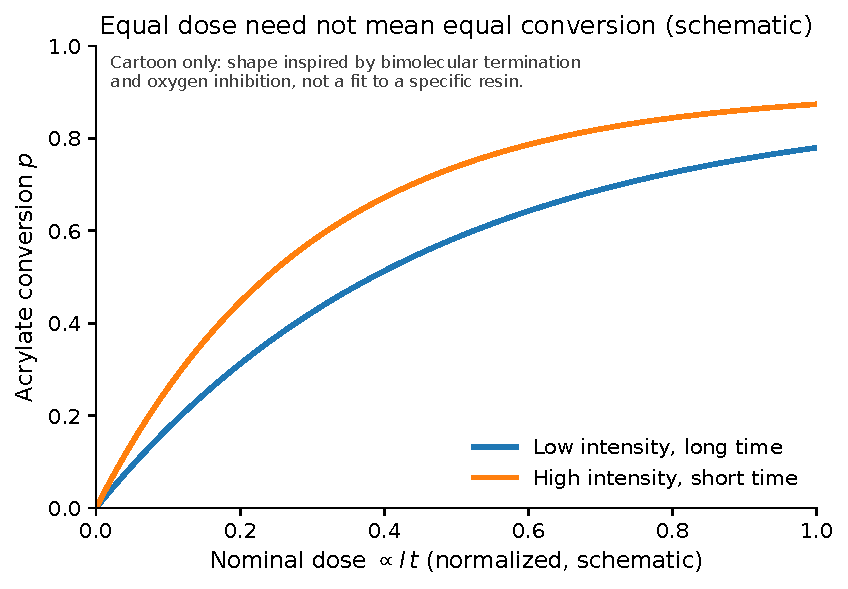
\includegraphics[width=0.82\textwidth]{fig_background_reciprocity.pdf}
  \caption{Schematic only.
  Two protocols with the same nominal dose need not yield the same conversion when termination is bimolecular and oxygen participates \citep{Wydra2014,Lin2019,Dobson2024}.
  The curves are not experimental measurements.}
  \label{fig:reciprocity}
\end{figure}

\section{Light as a field in a participating medium}

Irradiance is not a property of the lamp alone.
It is a field $I(\mathbf{x},t)$ inside an absorbing (and sometimes scattering) mixture.

\subsection{Beer--Lambert attenuation that evolves with chemistry}

If scattering and emission are negligible and the beam is treated as unidirectional, a steady radiative balance reduces to
\begin{equation}
  \frac{\partial I}{\partial z} + A(\mathbf{x},t)\,I = 0,
  \label{eq:beer}
\end{equation}
with $z$ along the beam \citep{Montgomery2022}.
The attenuation $A$ is a sum of contributions: remaining photoinitiator, unreacted monomer, polymer, and any dedicated absorber dye.
As initiator is consumed, $A$ can fall (\emph{photobleaching}, especially for Type~II dyes \citep{Zhu2020}).
As polymer forms, $A$ can rise if the polymer absorbs more than the monomer \citep{Montgomery2022}.
In an optically thick sample the result is a polymerization \emph{front} that advances from the illuminated face \citep{Cabral2005,Zhu2020}.

Equation~\eqref{eq:beer} is already an engineering reduction of radiative transfer.
It is appropriate for a clear PEGDA resin.
It is not appropriate for a ceramic-filled slurry, where scattering dominates.

\subsection{Pixels, grayscale, and the point-spread function}

A digital micromirror device (DMD) does not paint a perfectly sharp bitmap onto the resin.
Each micromirror illuminates a small neighbourhood.
\citet{Montgomery2022} represent that neighbourhood as a Gaussian and obtain the surface irradiance by summing all pixels, including grayscale (partial on-time of a mirror).
\citet{Meenakshisundaram2020} insist that the true kernel need not be Gaussian: measured irradiance from a projection head can have a flatter core and more bleed than a first-order Gaussian, because of mirror tilt, imperfect collimation, and the relay optics \citep[citing][]{Zhou2009}.

The ontology distinction:
\begin{itemize}
  \item the \emph{commanded bitmap} is a discrete pattern of grayscale values;
  \item the \emph{surface irradiance} is a continuous field obtained by convolution with the optical kernel and, if the head or the image moves, by a time integral;
  \item the \emph{in-resin irradiance} is that surface field after attenuation~\eqref{eq:beer};
  \item the \emph{chemical conversion} is the result of the kinetic skeleton driven by the in-resin irradiance.
\end{itemize}
Collapsing all four into a Jacobs working curve throws away the objects one needs in order to predict grayscale gradients and overcure \citep{Montgomery2022,Meenakshisundaram2020}.

\section{Two independent motions}

It is easy to say ``the process is moving.''
Two different velocities must be named (Fig.~\ref{fig:vel}).

\begin{figure}[htbp]
  \centering
  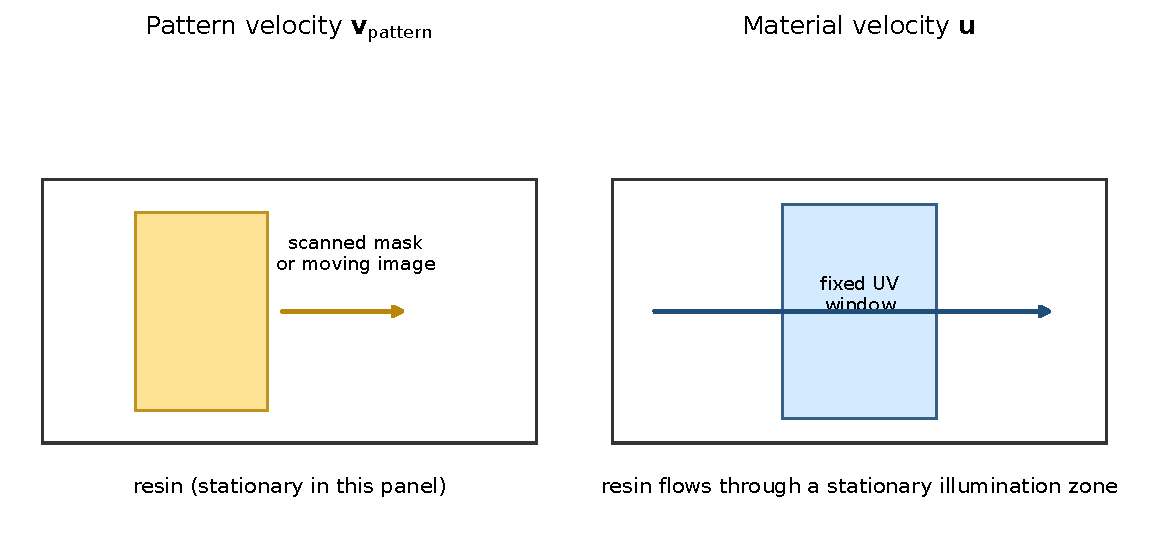
\includegraphics[width=0.98\textwidth]{fig_background_two_velocities.pdf}
  \caption{Left: the illumination pattern moves over a vat (scanning mask or scrolled image) while the resin is, to first approximation, still \citep{Meenakshisundaram2020}.
  Right: the resin flows through a fixed light window \citep{Slutzky2019}.
  A fluid element experiences the \emph{relative} motion of pattern and material.}
  \label{fig:vel}
\end{figure}

\paragraph{Pattern velocity $\mathbf{v}_{\mathrm{pattern}}$.}
In scanning-mask projection, the projector (or the bitmap on the DMD) translates so that a large area can be addressed with a small chip \citep{Meenakshisundaram2020}.
Frame rate, scan speed, and projected pixel pitch together decide how long a resin point sees each column of the movie.
One can even scroll the bitmap to \emph{cancel} stage motion, so that a feature is stationary in the vat while the hardware moves.

\paragraph{Material velocity $\mathbf{u}$.}
In a microfluidic jet, oligomer is carried through a stationary UV spot of length $L$ at speed $U$ \citep{Slutzky2019}.
The residence time in the light is $t_L = L/U$.
If the lamp is pulsed for a duration $t_{\mathrm{uv}}$, the relevant dimensionless exposure is $t_{\mathrm{uv}}/t_L$.

A material element at position $\mathbf{x}_p(t)$ with $\mathrm{d}\mathbf{x}_p/\mathrm{d}t=\mathbf{u}$ sees
\begin{equation}
  I_p(t) = I\bigl(\mathbf{x}_p(t),t\bigr).
\end{equation}
That sampled history is what the kinetic skeleton should be fed.
Calling both ``speed'' hides whether one is moving the lamp, the mask, or the liquid.

\section{Flow replenishes oxygenated resin}

In a closed, stagnant film, dissolved oxygen is a finite inventory (plus whatever diffuses from the walls).
In a continuous flow, fresh, oxygenated liquid continually enters the illumination zone.
\citet{Slutzky2019} make this the condition for fiber formation: polymerization remains negligible until oxygen is depleted, and the critical processing speed scales with how fast photolysis can eat the incoming $\mathrm{O}_2$ inventory,
\begin{equation}
  U_c \sim \frac{L\,\phi\,\varepsilon I\,[\mathrm{PI}]_0}{[\mathrm{O}_2]_0},
  \label{eq:Uc}
\end{equation}
up to the precise photophysical factors in their analysis.
They also argue that, for their jet diameter and speeds, oxygen \emph{diffusion into the jet during the residence time} is a small correction relative to advection of the dissolved inventory.
That statement is geometry-specific.
In a thin film against PDMS, the opposite limit can hold: diffusion from the wall dominates \citep{Dendukuri2008}.

The ontology: \emph{advection} and \emph{diffusion} of oxygen are different supply routes.
A model that includes only one of them is answering a different experiment.

\section{Conversion is not gelation is not modulus}

Figure~\ref{fig:stack} is the single most important hierarchy in this note.

\begin{figure}[htbp]
  \centering
  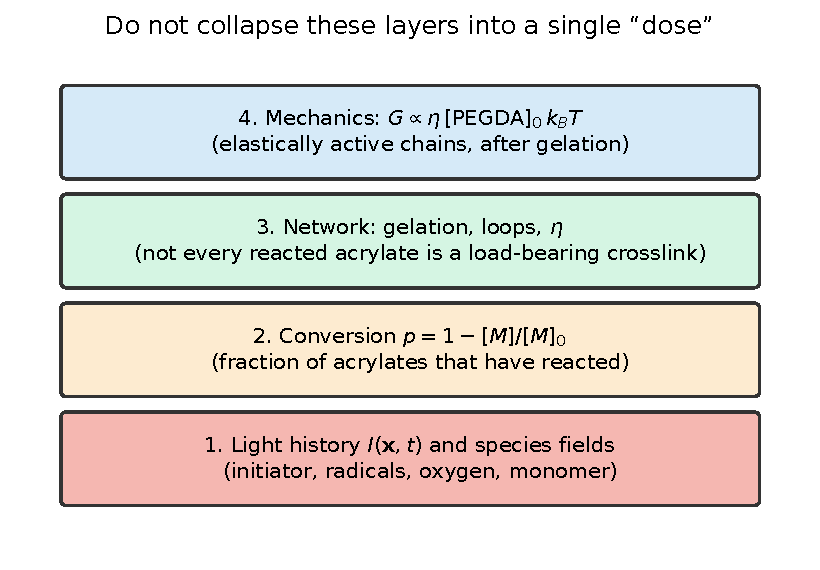
\includegraphics[width=0.88\textwidth]{fig_background_network_stack.pdf}
  \caption{Four layers that must not be identified.
  Light history and species fields determine conversion $p$; $p$ and composition determine whether a sample-spanning network exists and how many chains are elastically active; modulus is a mechanical consequence of that network \citep{Zhu2020,Macosko1976,Zhong2016}.}
  \label{fig:stack}
\end{figure}

\subsection{Gelation}

Gelation is the appearance of a sample-spanning covalently connected cluster: the weight-average molecular weight diverges \citep{Flory1941,Macosko1976}.
For a chain-growth polymerization of a multifunctional acrylate, that can occur at \emph{low} conversion because each chain can connect many monomers.

Two operational definitions in the present corpus must not be mixed without comment.

\begin{itemize}
  \item \citet{Slutzky2019} take gelation, following earlier microfluidic work, when about $2\%$ of double bonds have reacted ($[M]/[M]_0=0.98$).
    That is a convenient kinetic threshold for ``the jet no longer behaves as a liquid'' under their conditions.
  \item \citet{Zhu2020} compute a conversion at gelation from a recursive Macosko--Miller argument that includes intramolecular loops.
    If $\theta$ is the probability that a reacted acrylate connected \emph{inter}molecularly rather than as a loop, then
    \begin{equation}
      P_{\mathrm{gel}} = \frac{1-\theta}{2\theta},
      \qquad
      \theta = \frac{[\mathrm{PEGDA}]_0}{[\mathrm{PEGDA}]_0 + 2C_0},
      \label{eq:pgel}
    \end{equation}
    so $P_{\mathrm{gel}} = C_0/[\mathrm{PEGDA}]_0$.
    If the precursor is more dilute than $C_0$, $P_{\mathrm{gel}}\ge 1$: the sample never gels even at full acrylate conversion, because too many additions are wasted as loops.
\end{itemize}

Both can be legitimate.
They are not the same predicate.

\subsection{Loops and elastically active density}

Even after gelation, not every reacted acrylate contributes a load-bearing chain.
An intramolecular loop links a strand to itself and does not transmit stress the way an intermolecular crosslink does \citep{Zhong2016,Zhu2020}.
\citet{Zhu2020} construct a fractional crosslinking density $\eta$ from the probabilities that arms lead to the infinite network, and then write a phantom-network shear modulus
\begin{equation}
  G = \eta\,N_A\,[\mathrm{PEGDA}]_0\,k_B T.
  \label{eq:G}
\end{equation}
The ideal affine or phantom network without loops is an upper bound; real PEGDA gels sit below it.
Fitting $G$ as a smooth function of dose, skipping $\eta$, hides the concentration-dependent gel point that \citet{Zhu2020} used to design stiffness gradients.

\subsection{Heat, shrinkage, and swelling}

Polymerization is exothermic; thick or intensely illuminated samples heat, and rates depend on temperature \citep{Goodner2002,Dobson2024}.
Conversion also shrinks the volume and, in hydrogels, the network later imbibes solvent.
Those are real couplings.
They are \emph{downstream} of a trustworthy conversion field.
Treating them as the first objects to predict, before $p(\mathbf{x},t)$ is even defined, inverts the hierarchy of Fig.~\ref{fig:stack}.

\section{How the five campaign papers partition the ontology}

The local literature folder is not five versions of one model.
Each paper owns a different layer.

\begin{table}[htbp]
\centering
\caption{Division of labour among the five unique reports in the campaign corpus.
``Owns'' means: this is the layer the paper actually closes with equations and experiments.
It does not mean the other layers are false.}
\label{tab:papers}
\small
\begin{tabular}{@{}p{0.28\textwidth}p{0.62\textwidth}@{}}
\toprule
Report & Layer owned \\
\midrule
\citet{Dobson2024} &
High-resolution kinetic ontology: many species, free-volume transport, short versus long radicals, oxygen, heat, one- and three-dimensional balances.
Chemistry illustrated on HDDA, not PEGDA.
\\
\citet{Montgomery2022} &
Spatial grayscale printing: four tracked species, conversion-dependent $k_p$ and $k_t$, evolving Beer--Lambert field, pixel overlap, lateral diffusion that blurs commanded edges.
PEGDA~$250$ / Irgacure~819.
\\
\citet{Meenakshisundaram2020} &
Projection kinematics: measured (possibly non-Gaussian) pixel irradiance, scanning mask, discrete frames, dose accumulation.
Cure profile compared to printed dimensions; chemistry is not the species skeleton above.
\\
\citet{Slutzky2019} &
Flowing material through a fixed light window: advection of initiator, radicals, monomer, and oxygen; critical speed; pulse duration versus residence time.
PEGDA~$575$ jet; oxygen diffusion into the jet argued small.
\\
\citet{Zhu2020} &
Type~II eosin~Y bleaching plus conversion-to-gelation-to-modulus closure with loops.
Frontal photopolymerization in depth.
PEGDA~$575$ hydrogel; no advection.
\\
\bottomrule
\end{tabular}
\end{table}

A predictive description of a \emph{flowing grayscale PEGDA hydrogel} needs all four chemical--physical layers---kinetics, optics, transport, network---but it should inherit each layer from the paper that actually resolved it, not average their rate constants.

\section{What must not be identified}

For a masters-level reader, the practical discipline is a list of forbidden equivalences.

\begin{enumerate}
  \item $E=\int I\,\mathrm{d}t$ $\not\equiv$ conversion $p$. Reciprocity fails when termination is bimolecular and oxygen participates \citep{Wydra2014,Lin2019}.
  \item Commanded bitmap $\not\equiv$ surface irradiance $\not\equiv$ in-resin $I(\mathbf{x},t)$ \citep{Meenakshisundaram2020,Montgomery2022}.
  \item Pattern velocity $\not\equiv$ resin velocity \citep{Meenakshisundaram2020,Slutzky2019}.
  \item Dissolved oxygen inventory $\not\equiv$ oxygen leaking through a wall \citep{Slutzky2019,Dendukuri2008}.
  \item Type~I photolysis $\not\equiv$ Type~II dye/amine bleaching \citep{Dadashi2016,Zhu2020,Montgomery2022}.
  \item PEGDA~$250$ in a dry thin film $\not\equiv$ PEGDA~$575$ in water $\not\equiv$ HDDA bulk \citep{Montgomery2022,Zhu2020,Dobson2024}.
  \item Acrylate conversion $p$ $\not\equiv$ gelation $\not\equiv$ elastically active density $\eta$ $\not\equiv$ modulus $G$ \citep{Zhu2020,Flory1941,Zhong2016}.
  \item A $2\%$ double-bond threshold \citep{Slutzky2019} $\not\equiv$ the Macosko--Miller $P_{\mathrm{gel}}([\mathrm{PEGDA}]_0)$ \citep{Zhu2020}.
  \item Chain-growth acrylate kinetics $\not\equiv$ thiol--ene step growth \citep{Cramer2001}.
  \item Jacobs working-curve depth \citep{Jacobs1992book} $\not\equiv$ a species-resolved polymer state.
\end{enumerate}

\section{Implications for a predictive description}

The ontology above already implies an order of questions, still without reference to implementation.

\begin{enumerate}
  \item \textbf{Local constitutive response.}
    For a prescribed $I(t)$, how do initiator, radicals, oxygen, and acrylate evolve?
    This is the question \citet{Dobson2024} answer at high chemical resolution and \citet{Montgomery2022} answer with four species and conversion-dependent coefficients.
    Until this map is trusted---including an equal-dose test that is \emph{allowed to fail}---spatial complexity only conceals error.
  \item \textbf{Optical boundary condition.}
    What irradiance actually sits on $z=0$ as a function of bitmap, pixel kernel, and pattern motion \citep{Meenakshisundaram2020}?
    Then, how does $A(p,[\mathrm{PI}])$ carry that field into the depth \citep{Montgomery2022,Zhu2020}?
  \item \textbf{Transport.}
    Which species move relative to the material?
    Oxygen almost always does; monomer may; network-bound radicals do not \citep{Dobson2024,Montgomery2022}.
    Is the supply advective \citep{Slutzky2019} or diffusive from a wall \citep{Dendukuri2008}?
  \item \textbf{Network closure.}
    Given $p$ and composition, has the sample gelled, and what is $\eta$ and $G$ \citep{Zhu2020}?
    This step must not be used to patch kinetic coefficients.
\end{enumerate}

The campaign choice that follows from this background is conservative: treat PEGDA chain-growth as the first chemical object; treat Dobson's full species set as a \emph{reference} against which reduced $k_p(p)$ and $k_t(p)$ can be judged, not as the first process model; treat scanning projection and plug flow as two different kinematic experiments; treat Zhu's loop-aware modulus as a post-processor on conversion.
Those are scientific restrictions, not software preferences.


\chapter{Literature study and research gaps}
\label{ch:literature}

\section{Scope of the corpus}

The working library comprises five unique journal papers, the supporting information of \citet{Dobson2024}, and a duplicate file of \citet{Meenakshisundaram2020} that must not be cited twice.
Supporting classics (oxygen inhibition, reciprocity, Macosko--Miller gelation, CLIP, frontal photopolymerization) are used as they appear in those reports, not as an unbounded review of photopolymer science.

The five papers do not compete to be ``the PEGDA model.''
Each \emph{owns a layer} (Table~\ref{tab:papers} in Chapter~\ref{ch:background}).
A flowing grayscale hydrogel would need all layers, inherited from the paper that actually closed each one.

\section{High-fidelity kinetics: Dobson and Bowman}

\citet{Dobson2024} construct a first-principles description of multifunctional acrylate photopolymerization with a large species set: photoinitiator, primary radicals, short and network-bound macroradicals, unreacted and partially reacted monomer, oxygen, and terminated polymer.
Mobility is tied to free volume; termination includes reaction-diffusion control and chain-length effects; heat release is optional.
The illustrated chemistry is 1,6-hexanediol diacrylate (HDDA) with Irgacure~819, not PEGDA.

The campaign uses this paper as a \emph{reference ontology}, not as production rates.
The temptation to ``implement Dobson first in 2-D'' is the usual way a PhD project becomes un-debuggable: too many species, too many spatial operators, and no algebraic limit that can fail loudly.
If, after a correct Montgomery transcription, equal-dose FTIR still cannot be organised, Dobson's chain-length $k_t$ is the parked refinement---not the first commit.

\section{Production spatial kinetics: Montgomery et al.}

\citet{Montgomery2022} is the production constitutive law for Type~I PEGDA~$250$ / 0.1~wt\% Irgacure~819 in a thin film.
Four species are tracked: initiator $C_I$, radicals $C_R$, oxygen $C_O$, monomer (acrylate groups) $C_M$.
With diffusion,
\begin{equation}
  \partial_t C_\alpha = \nabla\cdot\bigl(D_\alpha(p)\nabla C_\alpha\bigr) + R_\alpha,
\end{equation}
and $R_\alpha$ given by their Eqs.~16--19.
Photolysis is first order in remaining initiator, with $\beta=2.70\times10^{-3}\,\mathrm{s^2\,kg^{-1}}$ multiplying $I$ in $\mathrm{W\,m^{-2}}$ so that $\beta I$ is a frequency.
Two radicals are produced per cleavage ($m=2$).
Termination is $2k_t C_R^2$ plus oxygen inhibition $k_O C_O C_R$.

The closures (their Eqs.~22--27, Table~2) make $k_p$ and $k_t$ conversion-dependent:
\begin{align}
  k_p(p) &= \frac{k_{p0}}{1+(k_{p0}/k_{p,D0})\exp(c_p p)}, \\
  k_t(p) &= \Bigl[\tfrac{1}{k_{t,\mathrm{SD}}}+\tfrac{\exp(c_p p)}{k_{t,\mathrm{TD0}}}\Bigr]^{-1}
           + C_{RD}(1-p)k_p(p).
\end{align}
(The paper writes $\exp(cp)$ for $\exp(c p)$ with $c$ the relative viscosity coefficient.)
Harmonic liquid--solid diffusivities (Eq.~28, Table~3) drop by four orders of magnitude from liquid to solid.
Beer--Lambert attenuation (Eqs.~4--6) uses molar initiator absorptivity, polymer versus monomer absorption, and an optional photoabsorber term $w A_{\mathrm{abs}}$.

The optical boundary condition (Eq.~7) superposes Gaussians of radius $\sigma=17.7\,\mu\mathrm{m}$ on a $50\,\mu\mathrm{m}$ pixel pitch, with $I_{\mathrm{pixel}}=41.08\,\mathrm{W\,m^{-2}}$ and $I_{\mathrm{ideal}}=64\,\mathrm{W\,m^{-2}}$.
G0 is full intensity and G100 is dark.
Their multilayer prints with 0.06~wt\% absorber are a different optical depth than the FTIR cell.

\paragraph{What we did not take from this paper as gospel.}
The Gaussian kernel is a fallback, not a measured DMD map.
The linear G0--G100 map used in code is \emph{assumed}, not their SI RGB calibration.
Table~2 rates are a fit to one thin-film recipe; they are not universal PEGDA constants.
Dissolved oxygen is not a Table~2 entry; the campaign flags $C_{O,0}$ as \stillreq.

\section{Projection kinematics: Meenakshisundaram, Sturm and Williams}

\citet{Meenakshisundaram2020} model scanning-mask projection vat photopolymerization.
The scientific object is the surface irradiance and the accumulated dose under a measured (generally non-Gaussian) pixel kernel, discrete frames, and a scan velocity.
They compare a Jacobs-style cure overlay to printed dimensions; that overlay is a diagnostic, not a species conversion.

The campaign Stage~3 implements conservation and bleed tests on Montgomery's Gaussian as a \emph{stand-in}.
A \tagmatch{} on Stage~3 requires a camera or radiometer map of the projector actually used, or digitization of their measured PSF.
Scan dose scaling as $1/v$ is a dwell identity for a translating compact pattern, not a statement that $p$ is independent of speed.

\section{Plug flow: Slutzky, Stone and Nunes}

\citet{Slutzky2019} pass a sheathed aqueous jet of PEGDA~$575$ (54~vol\%), water, dye, and 4~vol\% 2-hydroxy-2-methylpropiophenone through a $L=2.3\,\mathrm{mm}$ UV slit.
Steady plug flow gives
\begin{equation}
  U\frac{\mathrm{d}C_i}{\mathrm{d}x}=R_i\bigl(C,k_d(x)\bigr),\qquad
  k_d=0\text{ outside }[0,L].
\end{equation}
Their Eqs.~1a--d use $k_d=\phi\varepsilon I$ with $I$ in Einstein~$\mathrm{m^{-2}\,s^{-1}}$, termination $k_t R^2$ (no extra factor of two), and one radical per photolysis as written in their Table~1.
Taking the ratio of monomer and oxygen balances at constant $k_p,k_O$ yields Eq.~3,
\begin{equation}
  \frac{C_O}{C_{O,0}}=\Bigl(\frac{C_M}{C_{M,0}}\Bigr)^{k_O/k_p}.
\end{equation}
Gelation for comparison to fiber onset is the operational predicate $M/M_0=0.98$ (about $2\%$ double bonds reacted), following microfluidic convention \citep{Dendukuri2008}---not Zhu's $P_{\mathrm{gel}}$.
Oxygen diffusion into the $40\,\mu\mathrm{m}$ jet during residence is argued small relative to advection of the dissolved inventory.

Critical speed scales as $U_c\sim L k_d [\mathrm{PI}]_0/[\mathrm{O}_2]_0$.
Pulsed light organises fiber length by $t_{\mathrm{uv}}/t_L$ with $t_L=L/U$.

This chemistry must not share a parameter book with Montgomery PEGDA~$250$/Irgacure.

\section{Network mechanics: Zhu et al.}

\citet{Zhu2020} couple Type~II eosin~Y / TEOA bleaching kinetics to acrylate conversion and then to a modified Macosko--Miller recursive model with intramolecular loops.
The campaign implements \emph{only} the network post-processor (their Eqs.~21, 26, 32--38).
Eosin bleaching ODEs (their Eqs.~3--8) remain off unless a Type~II kinetics branch is explicitly opened.

The intermolecular probability is
\begin{equation}
  \theta=\frac{[\mathrm{PEGDA}]_0}{[\mathrm{PEGDA}]_0+2C_0},
\end{equation}
with fitted $C_0=3.45$~vol\% (Table~A2).
Then $P_{\mathrm{gel}}=(1-\theta)/(2\theta)=C_0/[\mathrm{PEGDA}]_0$.
If $[\mathrm{PEGDA}]_0\le C_0$, the precursor never gels at $p=1$.
Without loops, $\eta=p^2$.
With loops, $\eta$ is assembled from probabilities that $m\ge 3$ carbon ends lead to the infinite network.
The phantom modulus is $G=\eta N_A[\mathrm{PEGDA}]_0 k_B T$, so $G/G_{\mathrm{ideal}}=\eta$.

\section{Supporting literature that the five papers rest on}

\paragraph{Oxygen.}
\citet{Decker1985} established the kinetic role of $\mathrm{O}_2$ as a radical scavenger.
\citet{Dendukuri2008} showed that PDMS walls replenish oxygen by diffusion and set a dead zone; that is a different experiment from Slutzky's jet.
\citet{Tumbleston2015} turned a persistent inhibited liquid layer into CLIP.

\paragraph{Reciprocity.}
\citet{Wydra2014} showed that BisGMA/TEGDMA does not obey $I\times t$ equivalence when bimolecular termination dominates.
\citet{Lin2019} organised related effects of oxygen, viscosity, and time-varying intensity.

\paragraph{Networks.}
\citet{Flory1941} and \citet{Macosko1976,Miller1976} are the gelation and post-gel recursive backbone.
\citet{Zhong2016} quantified how primary loops reduce elasticity.
\citet{Anseth1994} and \citet{Benson1959} frame diffusion-controlled termination.
\citet{Cabral2005} described light-driven polymerization fronts.
\citet{Goodner2002} coupled heat and mass transfer in thick films.
\citet{Dadashi2016} reviews Type~I versus Type~II initiation.
\citet{Cramer2001} marks thiol--ene as a different polymerization, parked here.

\section{Working curves, CLIP, and why they are not the polymer state}

Stereolithography practice has long used a working curve $C_d=D_p\ln(E/E_c)$ \citep{Jacobs1992book}.
$D_p$ is an effective optical penetration; $E_c$ is a critical exposure at which a gel-like depth is first observed for a given resin and process.
The construction is invaluable for machine calibration.
It collapses oxygen, termination order, grayscale bleed, and flow into two fitted numbers.
Those numbers change when the lamp spectrum, inhibitor, or speed changes, which is exactly the symptom that they are not constitutive.

Continuous liquid interface production \citep{Tumbleston2015} exploits a persistent oxygen-inhibited dead zone so that a part can be drawn continuously from a vat.
That dead zone is a \emph{diffusive} oxygen supply from a permeable window, closer in spirit to \citet{Dendukuri2008} than to \citet{Slutzky2019}, whose jet carries its oxygen inventory by advection.
A CLIP-style boundary condition is therefore a later Stage~4 variant, not a reason to replace $p$ with $C_d$.

Frontal photopolymerization \citep{Cabral2005} is another macroscopic signature of the same microscopic rates: an optically thick, exothermic film can propagate a conversion front.
Stage~4's Beer--Lambert front at $H=200\,\mu\mathrm{m}$ is a thin, isothermal cousin of that phenomenon, not a heat-release model \citep{Goodner2002}.

\section{Undermind synthesis versus what was coded}

A broader modelling note exists in the DFG Undermind workspace (unified photopolymerization roadmap and Stage~1 PEGDA implementation notes).
That synthesis is right about history-dependent kinetics, independent pattern and resin velocities, and the need for a loop-aware network closure.

It is not internally consistent as an \emph{execution order}.
One passage suggests implementing Dobson first, or making the first solver two-dimensional with a measured PSF.
The Stage~1 PEGDA notes, by contrast, specify a local four-species ODE, BDF integration, and Dobson as a check.

The code follows the Stage~1 notes and the local five-PDF ladder.
Undermind extras (Dendukuri walls, Wydra named tests, four in-house reactors, $\sim 80\,\mu\mathrm{m}$ flowing DMD patches) are treated as future \emph{tests and boundary conditions}, not as extra architecture in Stages~0--6.

\section{The gap closed by this campaign}

Before this repository, the group had papers, not a citable stack.
The specific gap was operational:

\begin{enumerate}
  \item No provenance-locked parameter books, so Montgomery $\beta$ could silently be used with Slutzky Einstein intensities.
  \item No local ODE with named gates (dark $p=0$, positivity, failed reciprocity, oxygen induction).
  \item No constant-rate fork to test Slutzky Eq.~3 as an identity rather than a fitted curve.
  \item No projection engine that is forbidden from reporting conversion.
  \item No 1-D reaction--diffusion with the \emph{same} cell RHS as the ODE.
  \item No plug-flow solver on Slutzky's stoichiometry.
  \item No network post-processor that cannot retune $k_p$.
\end{enumerate}

The remaining gap is \emph{quantitative match} under the same formulation (Chapter~\ref{ch:matching}), plus parked physics (heat, scattering, NS--gel, inverse DMD).

\chapter{Software architecture and numerical methods}
\label{ch:methods}

\section{Design principles}

The package is a \emph{staged scientific solver}, not a printer controller.
Three principles are enforced in code and in process:

\begin{enumerate}
  \item \textbf{One chemistry key per constitutive law.}
    Montgomery Type~I PEGDA~$250$, Slutzky Type~I PEGDA~$575$ jet, and Zhu Type~II network parameters live in three JSON books.
    A driver that needs plug flow does not import Montgomery $k_p$.
  \item \textbf{Shared RHS where the claim is the same chemistry.}
    Stage~4's method of lines calls the same vectorized \texttt{reaction\_rates} as Stage~1.
    Stage~5 does \emph{not}: Slutzky's $k_d$, $k_t R^2$, and Einstein $I$ are a different stoichiometry.
  \item \textbf{Post-processors cannot retune rates.}
    Zhu $\eta(p)$ is a map from conversion already obtained.
    Projection cannot emit $p$.
\end{enumerate}

Python~\texttt{>=3.9} is required.
The installable layout is \texttt{package-dir=\{""="src"\}} in \texttt{pyproject.toml}; campaign drivers prepend \texttt{src/} to \texttt{sys.path} so a researcher can run without installing.
Dependencies are NumPy, SciPy, and Matplotlib; tests use pytest.

\section{Repository layout}

The scientific kernel lives under \texttt{src/photopolymerization/}:

\begin{verbatim}
src/photopolymerization/
  parameters.py          KineticParams, OpticalParams, books
  kinetics/
    rhs.py               Montgomery reaction_rates, ODE rhs
    closures.py          p, kp(p), kt(p)
    protocols.py         I(t) callables
    solve.py             scipy.integrate.solve_ivp BDF
    limits.py            QSS residual, Slutzky Eq. 3 residual
  projection/psf.py      Gaussian pixel kernel (no chemistry)
  rd/
    beer.py              Beer-Lambert A(p, C_I)
    diffusivity.py       harmonic D_i(p)
    operators.py         1-D conservative diffusion
    mol.py               method-of-lines RHS
    mms.py               cosine manufactured solution
    solve.py             BDF on stacked 4 n_z state
  flow/
    params.py            Slutzky jet book
    plug.py              U dy/dx = R(y; k_d(x))
  network/macosko.py     theta, P_gel, eta, G
\end{verbatim}

Campaign artefacts sit beside the kernel, not inside it:

\begin{verbatim}
campaigns/pegda/
  configs/               frozen JSON per stage + three books
  drivers/               run_*.py, validate_*.py
  tests/                 pytest gates (29 tests as of Stage 6)
outputs/                 gitignored CSV/HDF of a run
docs/figures/            overview PDFs committed as lab evidence
journal/entries/         one markdown file per stage
\end{verbatim}

\section{The campaign quartet}

Every stage $N\in\{0,\ldots,6\}$ produces the same four artefacts:

\begin{enumerate}
  \item \texttt{config.pegda\_stage$N$.json} --- frozen knobs for \emph{this} claim.
  \item \texttt{run\_pegda\_stage$N$.py} --- forward calculation and overview figure.
  \item \texttt{validate\_pegda\_stage$N$.py} --- named gates, \texttt{OVERALL PASS} or \texttt{FAIL}.
  \item \texttt{journal/entries/2026-09-13-pegda-stage$N$.md} --- one evidence tag.
\end{enumerate}

A pytest file \texttt{test\_pegda\_stage$N$.py} wraps the same gates so a regression cannot silently reopen a closed stage.
The process rule is to \textbf{stop} after a stage: engineering success (no \texttt{NaN}, finite $p$) is not a licence to couple Navier--Stokes.

\section{Parameter books}

\subsection{Montgomery 2022 (Type~I, PEGDA 250)}

File \texttt{parameter\_book.montgomery\_2022.json}.
Initiator loading $0.1$~wt\% Irgacure~819; $\beta=2.70\times10^{-3}\,\mathrm{s^2\,kg^{-1}}$ with $I$ in $\mathrm{W\,m^{-2}}$; $m=2$.
Table~2 closures $k_{p0}$, $k_{p,D0}$, $c_p$, $k_{t,\mathrm{SD}}$, $k_{t,\mathrm{TD0}}$, $C_{RD}$, $k_O$.
Calculated $C_{M0}=8880\,\mathrm{mol\,m^{-3}}$, $C_{I0}=2.651\,\mathrm{mol\,m^{-3}}$.
Dissolved oxygen $C_{O0}=1.0\,\mathrm{mol\,m^{-3}}$ is labelled \stillreq{}: it is a plausible order of magnitude, not a FTIR-fitted inventory.
Optical Table~1 coefficients and Table~3 liquid/solid diffusivities are attached for Stage~4 only.

\subsection{Slutzky 2019 (Type~I, PEGDA 575 jet)}

File \texttt{parameter\_book.slutzky\_2019.json}.
Window $L=2.3\,\mathrm{mm}$; Table~1 $k_p$, $k_t$, $k_O$; $k_d=\phi\varepsilon I$ with $I$ in Einstein~$\mathrm{m^{-2}\,s^{-1}}$.
Gel predicate $\min M/M_0\le 0.98$.
This book must never be mixed with Montgomery $\beta I$.

\subsection{Zhu 2020 (network only)}

File \texttt{parameter\_book.zhu\_2020.json}.
$C_0=3.45$~vol\% (Table~A2, \emph{fitted}).
Flag \texttt{eosin\_Y\_bleaching\_odes: off}.
Phantom $G$ uses an assumed PEGDA density to convert vol\% to $\mathrm{mol\,m^{-3}}$; ratios $G/G_{\mathrm{ideal}}=\eta$ are independent of that density.

\section{Time integration of the local ODE}

The Stage~1 state is $y=(C_I,C_R,C_O,C_M)$.
The system is stiff once radicals appear: photolysis and oxygen scavenging are fast relative to acrylate conversion.
The integrator is SciPy's \texttt{solve\_ivp} with method \texttt{BDF}, relative tolerance $10^{-6}$ and absolute tolerances that keep $C_R$ from being treated as zero while it is still chemically active.

A \texttt{constant\_rate=True} fork freezes $k_p=k_{p0}$ and $k_t=k_t(p=0)$.
That fork exists only so Slutzky Eq.~3 and a quasi-steady radical residual can be tested as \emph{identities}.
Production runs use the full $k_p(p)$, $k_t(p)$.

\section{Projection without chemistry}

Stage~3 evaluates Montgomery Eq.~7,
\begin{equation}
  I(x)=\sum_{\mathrm{on}} I_{\mathrm{pixel}}
  \exp\Bigl(-\Bigl(\frac{x-x_0}{2\sigma}\Bigr)^2\Bigr),
\end{equation}
with $\sigma=17.7\,\mu\mathrm{m}$, $I_{\mathrm{pixel}}=41.08\,\mathrm{W\,m^{-2}}$, pitch $50\,\mu\mathrm{m}$.
The 1-D integral of one Gaussian is $I_{\mathrm{pixel}}\,2\sigma\sqrt{\pi}$; the 2-D axisymmetric integral is $4\pi\sigma^2 I_{\mathrm{pixel}}$ for the written kernel.
Linear grayscale (G0 full, G100 dark) is an \emph{assumption} for tests, not a camera calibration.

\section{One-dimensional reaction--diffusion}

The stacked state is length $4n_z$.
Interior nodes use a conservative second-difference of $D_i(p)\partial_z C_i$.
Harmonic interpolation of $D_i$ follows Montgomery Eq.~28.
Beer--Lambert attenuation along $z$ uses
\begin{equation}
  A=\alpha_I C_I + p A_{\mathrm{poly}}+(1-p)A_{\mathrm{mon}}+w A_{\mathrm{abs}},
\end{equation}
with $w$ interpreted as weight percent as in their wording of Eq.~6.

An explicit Fourier time step $H^2/(2 n_z^2 \max D_i)$ is \emph{documented} as a CFL reference; the integrator remains implicit BDF.
A cosine manufactured solution with frozen $D_I^{\mathrm{liq}}$ checks the diffusion operator independently of chemistry.
Sealed Neumann boundaries conserve $\int C_M$ in the dark.
An oxygen Dirichlet node at the lit face is an inhibition-layer probe, not a CLIP printer.

\section{Plug-flow marching}

Stage~5 integrates
\begin{equation}
  U\frac{\mathrm{d}y}{\mathrm{d}x}=R\bigl(y;k_d(x)\bigr)
\end{equation}
with $y=(\mathrm{PI},R,y_{\mathrm{O_2}},M)$ in Slutzky's units.
Outside $[0,L]$, $k_d=0$.
The independent variable is $x$, not $t$; pulse lengths in the overview figure are kinematic $U t_{\mathrm{uv}}$.
A gate that PI is frozen for $x>L$ must sample with \texttt{searchsorted}, not \texttt{argmin} of $|x-L|$ (which can still lie inside the window).

\section{Network algebra}

Stage~6 evaluates Zhu's looking-out construction.
No ODE is integrated.
Montgomery $p(t)$ may be passed through $\eta(p)$ only if the plot is labelled \emph{hypothetical}: Type~I conversion is not Type~II eosin~Y conversion.

\section{Two Type~I right-hand sides that must not be merged}

Montgomery and Slutzky both describe Type~I chain growth, and both use a four-component state that looks like $(C_I,C_R,C_O,C_M)$.
They are nevertheless different constitutive laws.

\paragraph{Montgomery (Stages 1 and 4).}
Photolysis is $\mathrm{d}C_I/\mathrm{d}t=-\beta I C_I$ with $I$ in $\mathrm{W\,m^{-2}}$ and $m=2$ radicals per cleavage.
Termination is written $2k_t C_R^2$.
$k_p$ and $k_t$ depend on $p$.
Time is the independent variable.

\paragraph{Slutzky (Stage 5).}
Photolysis frequency is $k_d=\phi\varepsilon I$ with $I$ in Einstein~$\mathrm{m^{-2}\,s^{-1}}$, and $k_d=0$ outside the window.
The paper's Table~1 stoichiometry is used as written: one radical per photolysis in the radical balance, termination $k_t R^2$ without an extra factor of two.
Rates are constant (no $k_p(p)$).
The independent variable is $x$ at fixed $U$.

A shared function name \texttt{rhs} would have been a silent recipe mix.
The package therefore keeps \texttt{kinetics/rhs.py} and \texttt{flow/plug.py} as separate modules and refuses to load Montgomery $\beta$ into the jet book.

\section{What is deliberately absent}

There is no Navier--Stokes solver, no radiative transfer with scattering, no inverse grayscale optimizer, no Dobson free-volume species set in production, and no mixing of eosin bleaching into \texttt{reaction\_rates}.
Those absences are scope locks, not unfinished TODOs of Stages~0--6.

\chapter{Results of the staged campaign}
\label{ch:results}

This chapter reports what the solvers actually did.
Every numerical value is tagged by the stage that produced it.
Internal gates that passed are \tagvalid.
No row in Table~\ref{tab:stage-status} is \tagmatch.

\begin{table}[htbp]
\centering
\caption{Campaign status on 13 September 2026.
Internal \tagvalid{} is not a literature overlay.}
\label{tab:stage-status}
\small
\begin{tabular}{@{}clp{7.2cm}@{}}
\toprule
Stage & Tag & Claim in one sentence \\
\midrule
0 & \tagvalid & Every Montgomery coefficient has a source or a \stillreq{} flag. \\
1 & \tagvalid & Local Type~I ODE: dark $p=0$, failed reciprocity, oxygen induction. \\
2 & \tagvalid & Constant-rate fork satisfies Slutzky Eq.~3 and QSS radicals. \\
3 & \tagvalid & Gaussian pixels conserve analytic integrals; no chemistry. \\
4 & \tagvalid & 1-D RD + Beer--Lambert: front, dead zone, PSF-dominated strip. \\
5 & \tagvalid & Slutzky plug flow: Fig.~3 $M/M_0\simeq0.86$; $U_c$ scales with $k_d$. \\
6 & \tagvalid & Zhu loops: $P_{\mathrm{gel}}=C_0/c$; $\eta(p=1)=0.378$ at 20~vol\%. \\
\bottomrule
\end{tabular}
\end{table}

\begin{figure}[htbp]
  \centering
  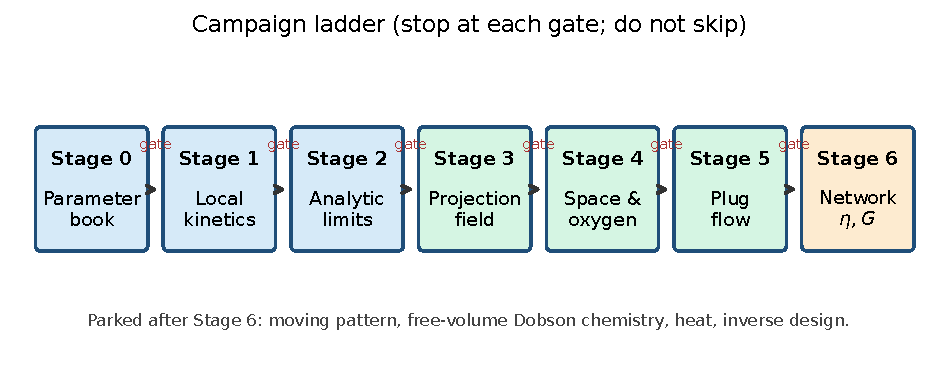
\includegraphics[width=0.92\textwidth]{fig_roadmap_stage_ladder.pdf}
  \caption{Locked stage ladder.
  Parked items (Dobson production RHS, NS--gel, inverse DMD, Type~II bleaching, Jacobs as polymer state) remain parked.}
  \label{fig:ladder}
\end{figure}

\section{Stage 0 --- provenance before kinetics}

The Montgomery book contains twenty entries with a chemistry key that forbids mixing with Zhu eosin~Y or Slutzky Einstein intensities.
$\beta$ is stored as $\mathrm{s^2\,kg^{-1}}$ so that $\beta I$ is a frequency when $I$ is in $\mathrm{W\,m^{-2}}$; using milliwatts per square centimetre without conversion would shift photolysis by a factor of ten.
$C_{O0}=1.0\,\mathrm{mol\,m^{-3}}$ is explicit and \stillreq.

\begin{figure}[htbp]
  \centering
  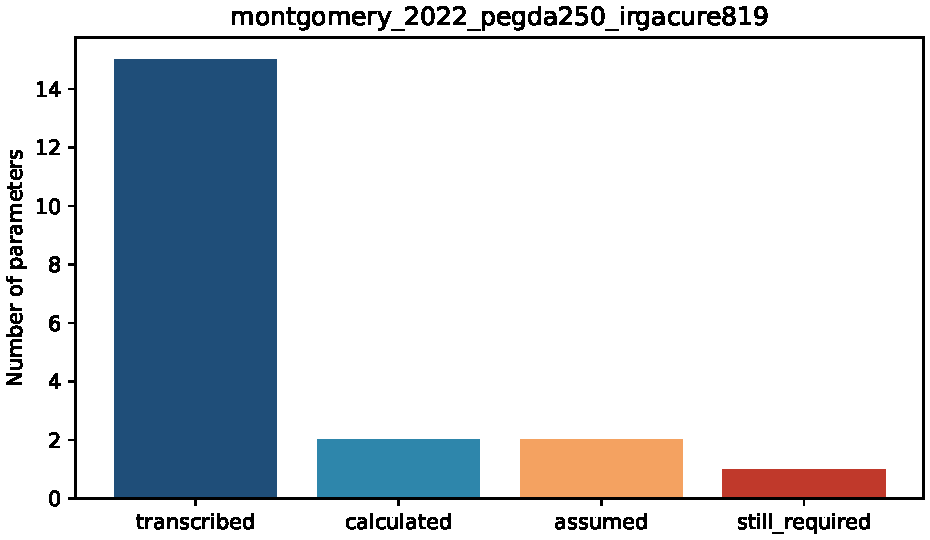
\includegraphics[width=0.88\textwidth]{pegda_stage0_overview.pdf}
  \caption{Stage~0 provenance overview (teaching layout of the book, not an experiment).}
  \label{fig:s0}
\end{figure}

\section{Stage 1 --- local Montgomery ODE}

With $I=0$, conversion remains $p=0$.
Species stay non-negative to a BDF floor of order $10^{-14}\,\mathrm{mol\,m^{-3}}$.
The acrylate integral residual against $\int R_p\,\mathrm{d}t$ is $\sim5\times10^{-5}$.
Equal dose does not give equal conversion: $64\,\mathrm{W\,m^{-2}}$ for $20\,\mathrm{s}$ yields $p=0.740$, while $16\,\mathrm{W\,m^{-2}}$ for $80\,\mathrm{s}$ yields $p=0.800$.
Oxygen delays the $p=0.02$ crossing from $0.90\,\mathrm{s}$ to $2.11\,\mathrm{s}$ under the assumed $C_{O0}$.

These numbers organise the \emph{sign} of reciprocity failure \citep{Wydra2014} and oxygen induction.
They are not a digitization of Montgomery's FTIR figure: intensity, film thickness, and dissolved oxygen of that figure were not re-fitted here.

\begin{figure}[htbp]
  \centering
  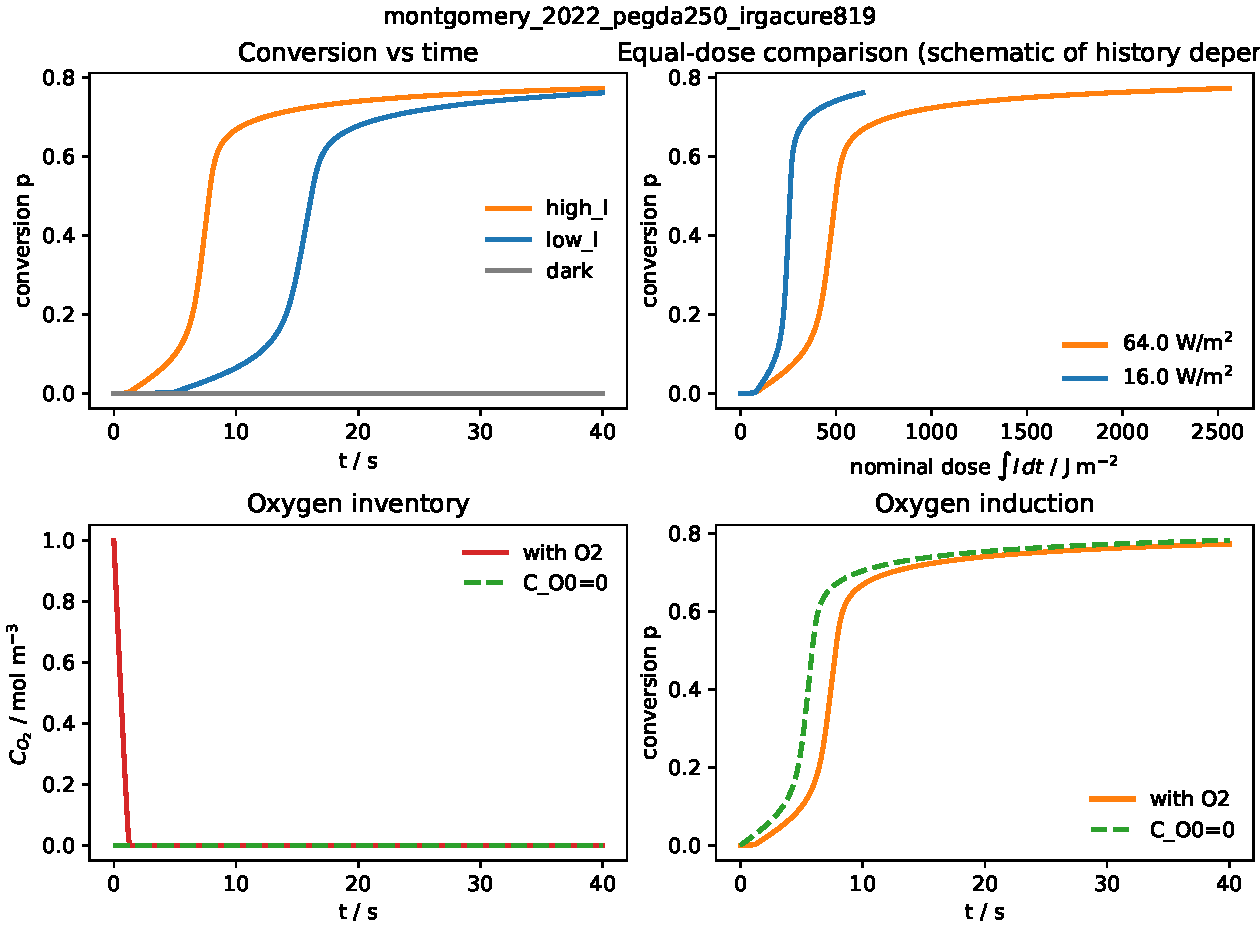
\includegraphics[width=0.95\textwidth]{pegda_stage1_overview.pdf}
  \caption{Stage~1 local ODE: conversion histories, equal-dose pair, and oxygen induction.}
  \label{fig:s1}
\end{figure}

\section{Stage 2 --- analytic identities on a constant-rate fork}

While $C_O/C_{O0}>0.05$, Slutzky Eq.~3 holds to a relative residual $1.12\times10^{-6}$ on the frozen-$k_p$ fork.
The same residual on the full Montgomery closures is $1.10\times10^{-6}$ in that window because $k_O/k_p\sim1.9\times10^3$ and conversion is still near zero.
The fork is chemically real later: $k_p(0.8)/k_p(0)=7\times10^{-4}$.
With $C_{O0}=0$, the quasi-steady radical residual against $\sqrt{R_i/2k_t}$ is $2.1\times10^{-3}$ after $0.5\,\mathrm{s}$.

Stage~2 is an identity test of the transcription.
It stays \tagvalid{} by construction; there is no laboratory overlay that would make it \tagmatch{} without confusing algebra with data.

\begin{figure}[htbp]
  \centering
  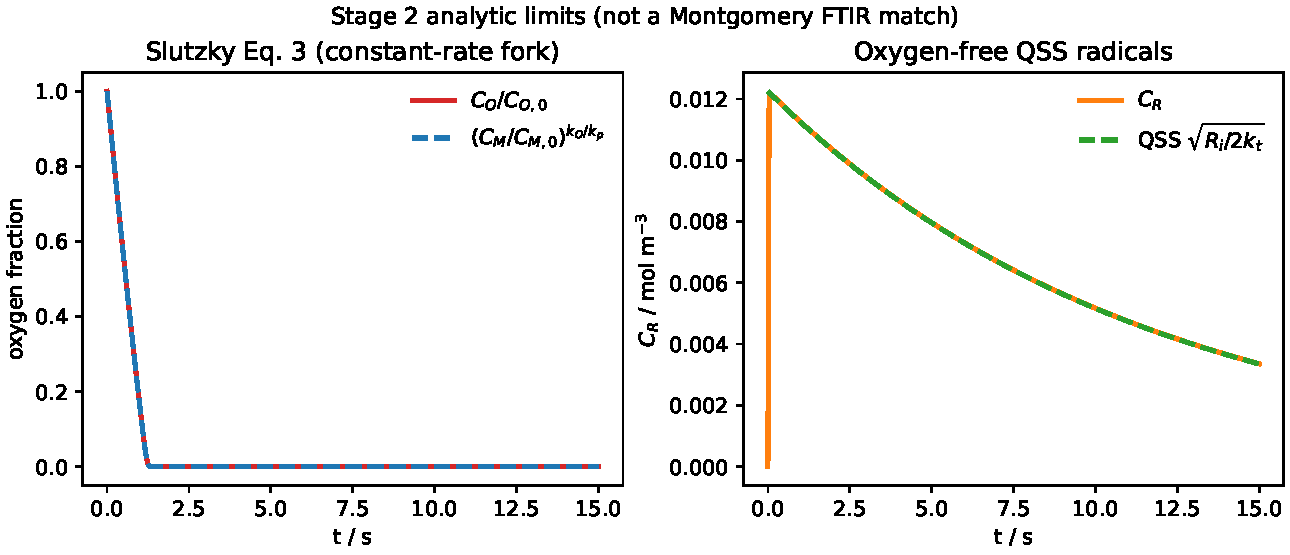
\includegraphics[width=0.95\textwidth]{pegda_stage2_overview.pdf}
  \caption{Stage~2: oxygen--monomer identity and quasi-steady radical residual.}
  \label{fig:s2}
\end{figure}

\section{Stage 3 --- Gaussian projection}

On a 1201-point line, the one-dimensional pixel integral matches $I_{\mathrm{pixel}}\,2\sigma\sqrt{\pi}$ to machine precision.
The two-dimensional integral matches $I_{\mathrm{pixel}}\,4\pi\sigma^2$ to $\sim10^{-16}$.
A dark bitmap is identically dark.
A ten-pixel block bleeds: edge $25.4\,\mathrm{W\,m^{-2}}$, interior $50.8\,\mathrm{W\,m^{-2}}$.
Scan dose peaks scale as $1/v$ to $2\times10^{-2}$ relative.

The integral of $I$ is \emph{not} $I_{\mathrm{pixel}}$ times the geometric pixel area $(50\,\mu\mathrm{m})^2$, because the written kernel is a Gaussian of width $\sigma$, not a top-hat of the pitch.
G0/G100 linearity is assumed.
A measured PSF \citep{Meenakshisundaram2020} is still required for \tagmatch.

\begin{figure}[htbp]
  \centering
  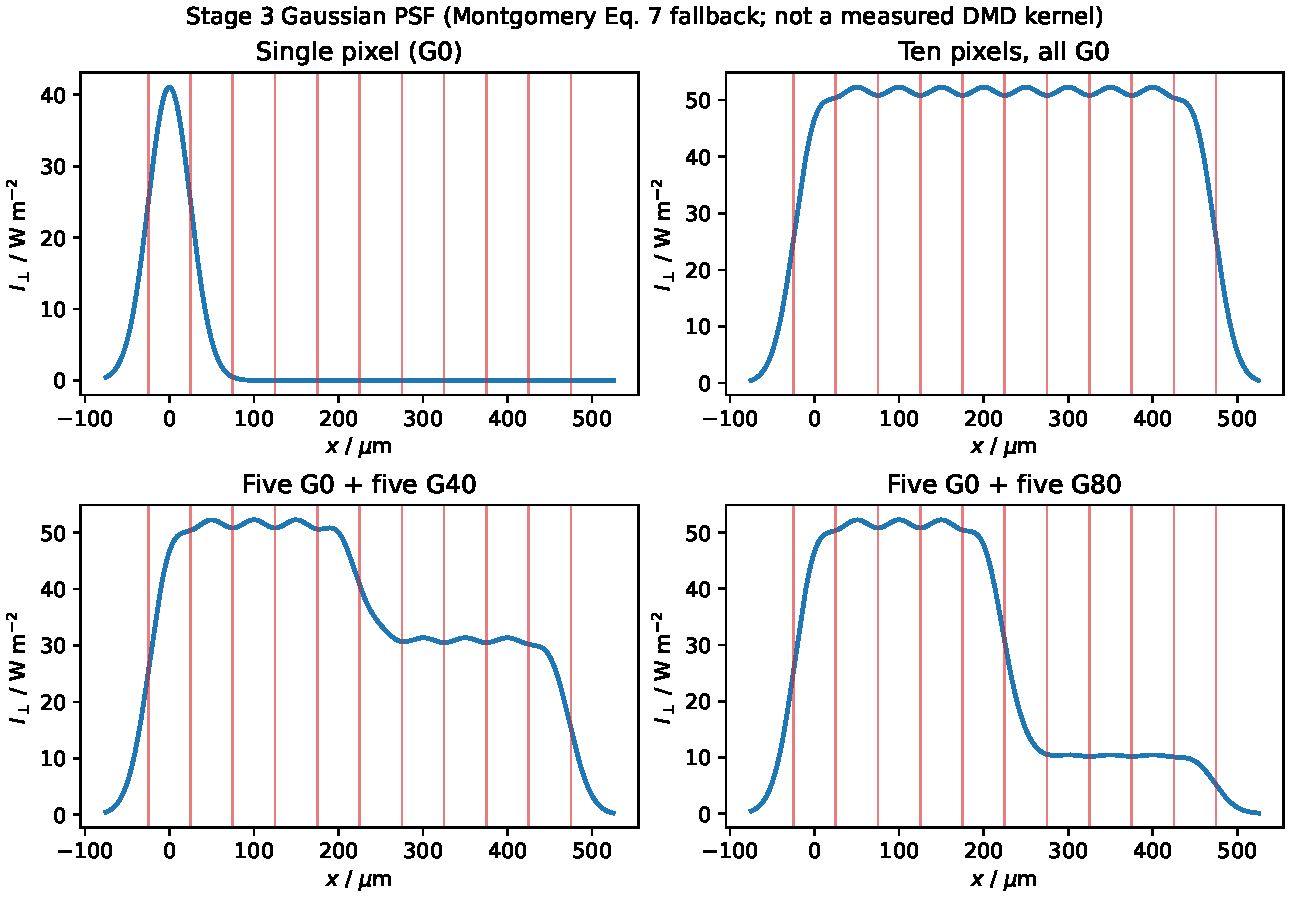
\includegraphics[width=0.95\textwidth]{pegda_stage3_overview.pdf}
  \caption{Stage~3 Gaussian projection (Montgomery Eq.~7 fallback). No conversion is plotted.}
  \label{fig:s3}
\end{figure}

\section{Stage 4 --- reaction--diffusion and Beer--Lambert}

A surface cell with $D_i=0$ reproduces Stage~1 conversion to $|\Delta p|\sim4\times10^{-6}$ at $8\,\mathrm{s}$ and $I=64\,\mathrm{W\,m^{-2}}$, so the MOL chemistry is the ODE chemistry.
Dark sealed films conserve $\int C_M$ to a relative residual of zero.
A cosine manufactured solution with frozen liquid $D_I$ has relative max error $6.9\times10^{-3}$.

A labelled $H=200\,\mu\mathrm{m}$ film with $w=0.06$~wt\% absorber reaches optical thickness $\beta_{\mathrm{opt}}=1.50$ and $p(0)-p(H)=0.52$ at $8\,\mathrm{s}$.
That geometry is \emph{not} Montgomery's FTIR cell.
An oxygen Dirichlet condition at the lit face gives $p_{\mathrm{wall}}=0.0069$ versus $p_{\mathrm{mid}}=0.53$.

A G0$|$G80 conversion strip has 10--90\% width $53\,\mu\mathrm{m}$, larger than $\sigma=17.7\,\mu\mathrm{m}$.
Turning Table~3 diffusivities on versus off changes that width by only $0.21\,\mu\mathrm{m}$ at $8\,\mathrm{s}$.
The 2--3 pixel printed interface in Montgomery Fig.~7 is therefore consistent with a \emph{PSF-dominated} blur, not with radical diffusion as the leading length.
A campaign gate that demanded ``$D$ on $\gg$ $D$ off'' would have been scientifically false; it was replaced by ``width $>\sigma$'' plus a note.

There is no coupled $x$--$z$ print grid in this stage.

\begin{figure}[htbp]
  \centering
  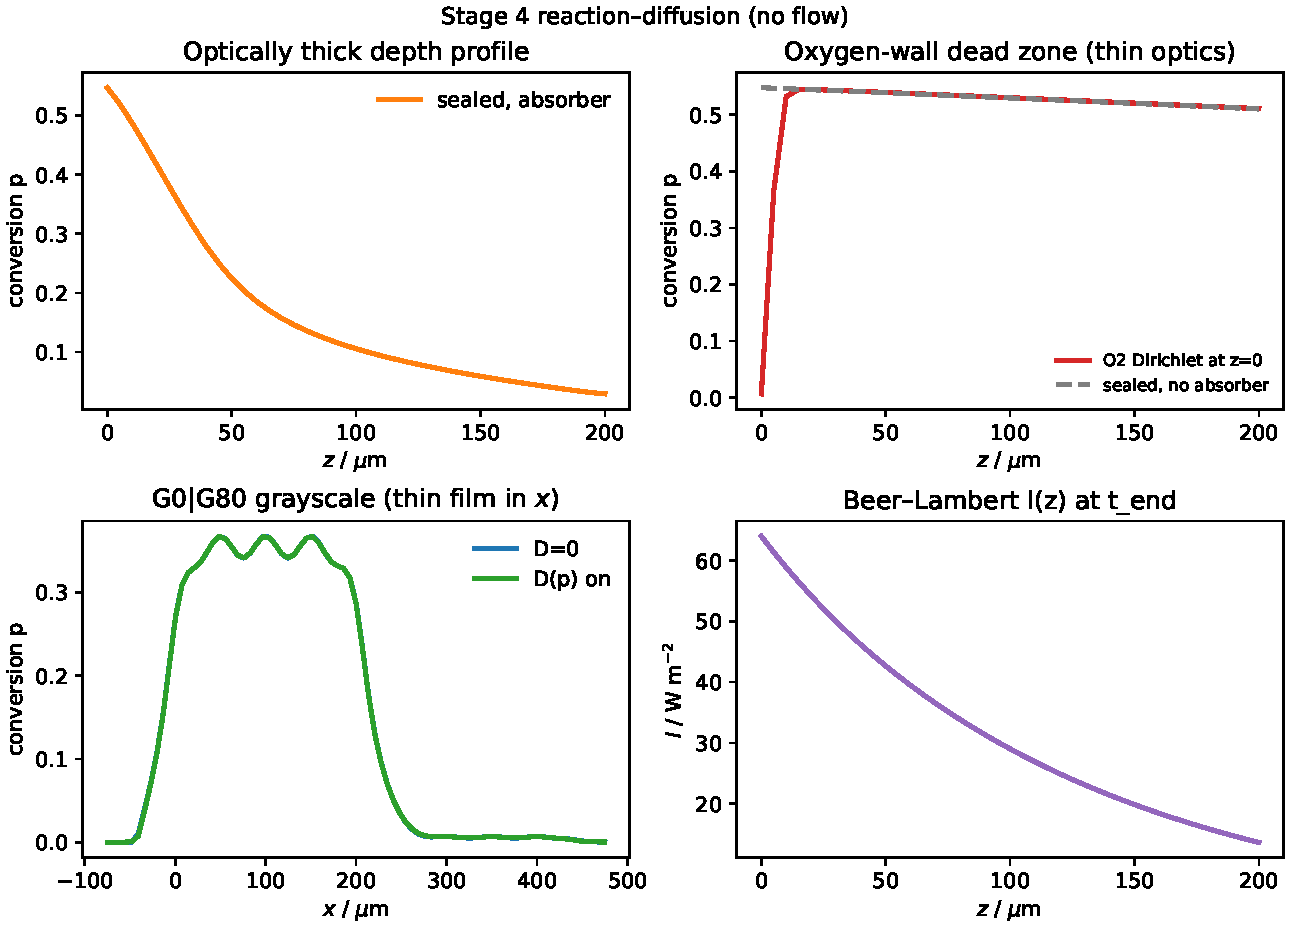
\includegraphics[width=0.95\textwidth]{pegda_stage4_overview.pdf}
  \caption{Stage~4: optical front, oxygen wall, and G0$|$G80 strip width.}
  \label{fig:s4}
\end{figure}

\section{Stage 5 --- Slutzky plug flow}

High-oxygen Fig.~2 parameters at $U=0.003\,\mathrm{m\,s^{-1}}$ keep $\min M/M_0=1.00$ (no gel under the 2\% predicate).
Low-oxygen Fig.~3 parameters reach $\min M/M_0=0.863$, against the paper's quoted $\simeq0.86$.
Eq.~3 along $x$ has residual $7.9\times10^{-7}$.
At $U=1\,\mathrm{m\,s^{-1}}$ the jet exits unconverted.
Quadrupling $k_d$ raises $U_c$ from $0.0018$ to $0.0072\,\mathrm{m\,s^{-1}}$; doubling $[\mathrm{PI}]_0$ raises $U_c$ from $0.0023$ to $0.0045\,\mathrm{m\,s^{-1}}$.

Pulse ``fiber'' lengths in the overview figure are $U t_{\mathrm{uv}}$, a kinematic construction, not a measured fiber campaign.
Wall oxygen diffusion is off, following their $\sqrt{Dt}\ll w_1$ argument.
The gel predicate is Slutzky's $M/M_0=0.98$, not Zhu $P_{\mathrm{gel}}$.

\begin{figure}[htbp]
  \centering
  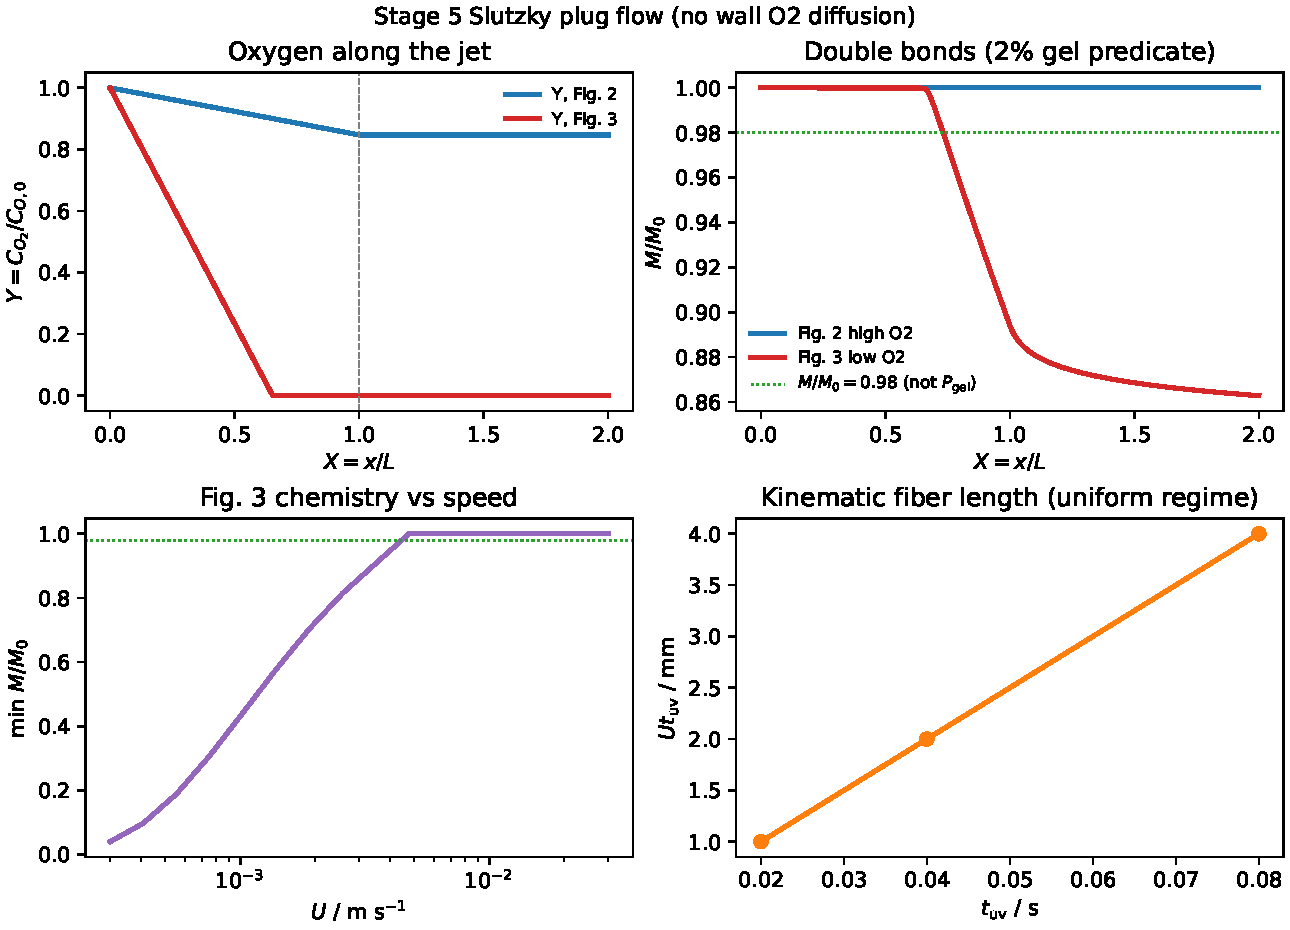
\includegraphics[width=0.95\textwidth]{pegda_stage5_overview.pdf}
  \caption{Stage~5 plug flow on the Slutzky book: conversion along $x$, $U_c$ trends, pulses.}
  \label{fig:s5}
\end{figure}

\section{Stage 6 --- Zhu network post-processor}

At $20$~vol\% PEGDA, $P_{\mathrm{gel}}=C_0/c=0.1725$.
If $c\le C_0$, $\eta(p=1)=0$: the precursor cannot gel.
The no-loop identity $\eta=p^2$ holds.
With loops at $20$~vol\% and $p=1$, $\eta=0.378=G/G_{\mathrm{ideal}}$.
Pregel $\eta=0$ for $p<P_{\mathrm{gel}}$.
$P_{\mathrm{gel}}=0.173$ is not Slutzky's 2\% double-bond operational gel.

Passing a Montgomery $p(t)$ through $\eta$ is labelled hypothetical: Irgacure Type~I conversion is not eosin~Y Type~II conversion.

\begin{figure}[htbp]
  \centering
  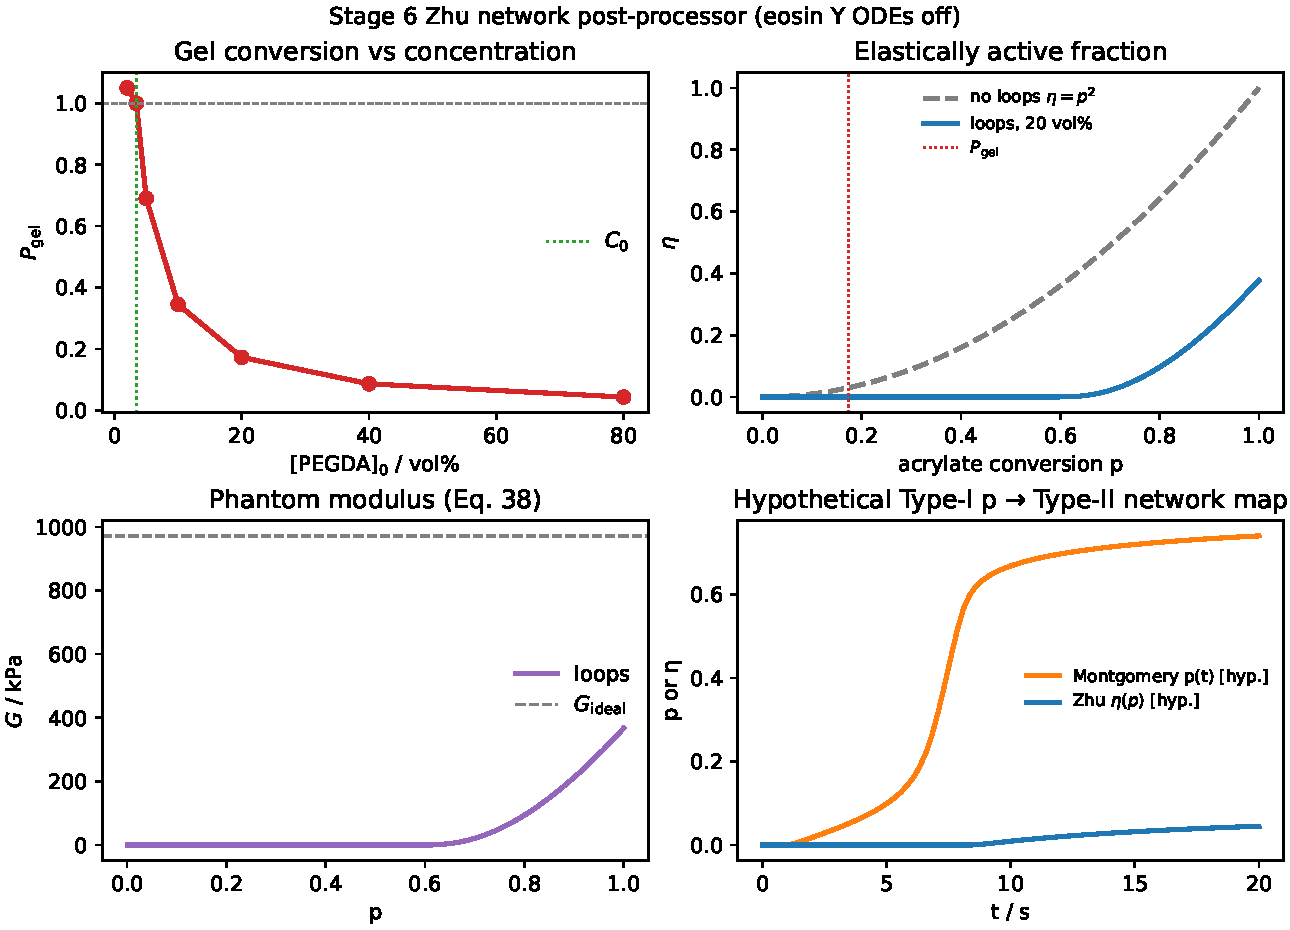
\includegraphics[width=0.95\textwidth]{pegda_stage6_overview.pdf}
  \caption{Stage~6 Macosko--Miller loops: $P_{\mathrm{gel}}(c)$, $\eta(p)$, and a hypothetical Montgomery trajectory.}
  \label{fig:s6}
\end{figure}

\section{Cross-stage reasonability}

Taken together, the stack behaves like photopolymerization rather than like a random ODE:

\begin{itemize}
  \item Dark resin does not convert.
  \item Oxygen delays conversion; fast flow can prevent gel under an operational $2\%$ threshold.
  \item Equal dose is not equal $p$ once $k_t$ is bimolecular and conversion-dependent.
  \item Pixels bleed; scan dose falls as $1/v$.
  \item Optically thick films convert more at the lit face; a Dirichlet $\mathrm{O}_2$ wall stays almost unconverted.
  \item Dilute PEGDA need not gel at $p=1$ if loops consume junctions.
\end{itemize}

None of those statements licenses transferring a fitted number across books.

\section{Tests}

As of Stage~6, \texttt{python3 -m pytest campaigns/pegda/tests -q} reports 29 passed.
Validators print \texttt{OVERALL PASS} on both \texttt{--smoke} and full modes for Stages~0--6.
Outputs under \texttt{outputs/pegda\_stage$N$\_out/} are gitignored; figures under \texttt{docs/figures/} are the citable lab plots.

\chapter{What would constitute a literature match}
\label{ch:matching}

A stage may be retagged \tagmatch{} only when a \emph{named number} from a \emph{named figure or table}, under the \emph{same formulation}, lies inside a \emph{pre-declared band}, and the validator plus journal are updated in the same commit of scientific record.

Matching is not ``the curve looks like polymerization.''
It is not transferring Montgomery $k_p$ onto a Slutzky jet.
It is not calling $M/M_0=0.98$ a Flory gel point.

\section{Recommended order}

\begin{enumerate}
  \item Stage~1 FTIR overlay (Montgomery PEGDA~$250$ / Irgacure~819).
  \item Stage~3 measured PSF (this projector, or Meenakshisundaram's map if claiming that printer).
  \item Stages~5 and~6 in parallel (different chemistries; no shared $k_p$).
  \item Stage~4 last, after the PSF is honest: otherwise a wrong kernel will be absorbed into $D_R$.
\end{enumerate}

Stage~2 remains \tagvalid{}: it is an identity, not a laboratory object.

\section{Stage 1}

Digitize Montgomery FTIR $p(t)$ at their reported $I$ and film.
Declare a band (for example $\max|p_{\mathrm{sim}}-p_{\mathrm{FTIR}}|<0.05$ on the illuminated window, or a tighter band on the induction time).
Measure or independently estimate $C_{O0}$; do not hide oxygen as a free fit that also absorbs errors in $\beta$.
Run the equal-dose pair at \emph{their} two intensities, not only at $64$ and $16\,\mathrm{W\,m^{-2}}$.

In-house AVT resin is a \emph{new book}, not a Montgomery match.

\section{Stage 3}

Replace Eq.~7 with a camera or radiometer single-pixel map, or digitize the measured kernel in \citet{Meenakshisundaram2020} if that is the claimed device.
If grayscale G0--G100 is claimed against Montgomery Fig.~3, transcribe their SI RGB$\to I$ calibration; do not keep the linear placeholder.

\section{Stage 4}

Only after Stage~3.
Compare a print geometry they actually used (layer height, absorber loading, grayscale pair) to Fig.~7 interface width.
Do not inflate $D_R$ to manufacture a $100$--$150\,\mu\mathrm{m}$ chemical blur that Table~3 plus an $8\,\mathrm{s}$ strip does not produce.

Dendukuri PDMS-wall dead zones are a different experiment (permeable walls, different resin).
They may become a later boundary-condition test, not a Montgomery match.

\section{Stage 5}

Overlay experimental $U_c(I,[\mathrm{PI}]_0)$ and fiber length versus $t_{\mathrm{uv}}/t_L$ from \citet{Slutzky2019} on the \emph{Slutzky} book.
The numerical Fig.~3 $M/M_0\simeq0.86$ is encouraging but is still an ODE illustration until the critical-speed map is overlaid with a declared band.

\section{Stage 6}

Overlay $G(p)$ or $G/G_{\mathrm{ideal}}$ versus $[\mathrm{PEGDA}]_0$ from \citet{Zhu2020} on the eosin~Y aqueous gel.
Do not call a hypothetical Montgomery $p\to\eta$ curve a Zhu match.

\section{Forbidden upgrades}

\begin{itemize}
  \item Matching Stage~1 never upgrades Stage~6.
  \item Matching Stage~5 never upgrades Stage~1.
  \item A Jacobs working curve overlay never upgrades conversion.
  \item A pretty $G(t)$ from mixing Type~II bleaching into Type~I rates is \taginvalid.
\end{itemize}

\chapter{Conclusions, limitations, and parked work}
\label{ch:conclusions}

\section{What this campaign established}

A citable Python stack now exists in which PEGDA Type~I conversion, Gaussian projection, one-dimensional reaction--diffusion, plug flow, and loop-aware network mechanics are \emph{separate claims} with frozen books and named gates.
Stages~0--6 are internally \tagvalid.
The chemical ontology of Chapter~\ref{ch:background} is enforced in code: dose is not conversion; conversion is not gelation; gelation is not modulus; Type~I is not Type~II; Montgomery PEGDA~$250$ is not Slutzky PEGDA~$575$; Slutzky's $2\%$ operational gel is not Zhu $P_{\mathrm{gel}}$.

The most important \emph{scientific} (not merely numerical) findings among the internal gates are:

\begin{enumerate}
  \item Equal-dose reciprocity already fails in the Montgomery closures at the two intensities tested.
  \item Slutzky Eq.~3 is an identity of constant $k_O/k_p$ during induction, recovered both in time (Stage~2) and along a jet (Stage~5).
  \item At Table~3 diffusivities and $8\,\mathrm{s}$, radical diffusion does not set grayscale feature size; the Gaussian PSF does.
  \item A 20~vol\% PEGDA network with Zhu's fitted $C_0$ reaches only $\eta=0.378$ at full conversion; below $C_0$ it never gels.
\end{enumerate}

\section{Limitations}

No FTIR, camera PSF, critical-speed map, or rheology overlay has been performed.
$C_{O0}$ remains assumed.
The Gaussian kernel and linear grayscale are placeholders.
Stage~4 is one-dimensional.
Stage~5 pulse lengths are kinematic.
Stage~6 $G$ uses an assumed density for absolute pascals; only $G/G_{\mathrm{ideal}}$ is density-free.
The Montgomery $p\to\eta$ plot is a thought experiment.

The literature study is bounded by the campaign PDFs plus the classics those papers cite.
It is not a complete review of stereolithography, CLIP, two-photon lithography, or thiol--ene materials.

\section{Parked work (do not auto-start)}

Full Dobson species as a production RHS; Navier--Stokes coupled to gelation; scattering; inverse DMD design; PNIPAM; thiol--ene; eosin~Y bleaching ODEs mixed into Irgacure Type~I; Jacobs depth as polymer state; four in-house reactors as extra architecture.

\section{Immediate scientific next step}

The first match attempt should be Stage~1: an FTIR $p(t)$ CSV on a named PEGDA / Type~I recipe, a declared error band, and a validator flag \texttt{--match} that cannot pass if the book chemistry key disagrees.
Until that exists, cite this report as a \emph{modelling and verification} thesis, not as a materials-property paper.

\chapter{Nomenclature}
\label{ch:nom}

Symbols are SI unless a paper uses Einstein units for photon flux; those cases are flagged in the Slutzky book.

\begin{table}[htbp]
\centering
\caption{Principal symbols.}
\label{tab:nom}
\small
\begin{tabular}{@{}llp{7.4cm}@{}}
\toprule
Symbol & Unit & Meaning \\
\midrule
$I$ & $\mathrm{W\,m^{-2}}$ or Einstein $\mathrm{m^{-2}\,s^{-1}}$ & Irradiance or molar photon flux \\
$E$ & $\mathrm{J\,m^{-2}}$ & Dose $\int I\,\mathrm{d}t$; not a material state \\
$p$ & --- & Acrylate conversion $1-C_M/C_{M0}$ \\
$C_I,C_R,C_O,C_M$ & $\mathrm{mol\,m^{-3}}$ & Initiator, radicals, oxygen, acrylate groups \\
$\beta$ & $\mathrm{s^2\,kg^{-1}}$ & Montgomery photolysis coefficient \\
$m$ & --- & Radicals per photolysis ($m=2$ Montgomery) \\
$k_p,k_t,k_O$ & various & Propagation, termination, oxygen scavenging \\
$A$ & $\mathrm{m^{-1}}$ & Beer--Lambert attenuation \\
$\sigma$ & $\mathrm{m}$ & Gaussian pixel radius (Montgomery Eq.~7) \\
$D_i(p)$ & $\mathrm{m^2\,s^{-1}}$ & Harmonic liquid--solid diffusivity \\
$U$ & $\mathrm{m\,s^{-1}}$ & Plug speed \\
$L$ & $\mathrm{m}$ & UV window length \\
$k_d$ & $\mathrm{s^{-1}}$ & Slutzky photolysis frequency $\phi\varepsilon I$ \\
$U_c$ & $\mathrm{m\,s^{-1}}$ & Critical speed for operational gel \\
$\theta$ & --- & Intermolecular linking probability \\
$C_0$ & vol\% & Zhu loop parameter (fitted 3.45~vol\%) \\
$P_{\mathrm{gel}}$ & --- & $C_0/[\mathrm{PEGDA}]_0$ \\
$\eta$ & --- & Elastically active density / $G_{\mathrm{ideal}}$ \\
$G$ & $\mathrm{Pa}$ & Phantom shear modulus \\
$\mathbf{v}_{\mathrm{pattern}}$ & $\mathrm{m\,s^{-1}}$ & Scan or mask velocity \\
$\mathbf{u}$ & $\mathrm{m\,s^{-1}}$ & Resin velocity \\
\bottomrule
\end{tabular}
\end{table}

\chapter{Appendix: verification log and file inventory}
\label{ch:app}

\section{How to reproduce the internal gates}

From the repository root, with Python~3.9+ and the dependencies in \texttt{pyproject.toml}:

\begin{verbatim}
export PYTHONPATH=src:campaigns/pegda
python3 campaigns/pegda/drivers/validate_pegda_stage0.py
python3 campaigns/pegda/drivers/validate_pegda_stage1.py
python3 campaigns/pegda/drivers/validate_pegda_stage2.py
python3 campaigns/pegda/drivers/validate_pegda_stage3.py
python3 campaigns/pegda/drivers/validate_pegda_stage4.py
python3 campaigns/pegda/drivers/validate_pegda_stage5.py
python3 campaigns/pegda/drivers/validate_pegda_stage6.py
python3 -m pytest campaigns/pegda/tests -q
\end{verbatim}

Each validator prints per-gate lines and \texttt{OVERALL PASS} or \texttt{FAIL}.
Smoke mode \texttt{--smoke} is a shorter integration window used in continuous checks.

\section{Overview figures}

Committed teaching and gate figures (all under \texttt{docs/figures/}):

\begin{itemize}
  \item background species, reciprocity, two-velocity, and network-stack cartoons;
  \item the stage-ladder diagram;
  \item \texttt{pegda\_stage0\_overview.pdf} through \texttt{pegda\_stage6\_overview.pdf}.
\end{itemize}

\section{Journal entries}

One markdown file per stage, all dated 13~September~2026, under \texttt{journal/entries/} with slugs \texttt{pegda-stage0} through \texttt{pegda-stage6}.
This thesis does not replace those entries; it synthesises them.

\section{What is gitignored}

Publisher PDFs in \texttt{Literature/} and numerical dumps in \texttt{outputs/} are local.
Do not redistribute publisher PDFs with this report.


\bibliographystyle{unsrtnat}
\bibliography{background_photopolymerization}

\end{document}
